\documentclass[UTF8,fontset=fandol,11pt,a4paper]{ctexart}
\usepackage[left=23mm,right=23mm,top=23mm,bottom=23mm,headheight=16pt]{geometry}
\usepackage{amsmath,amssymb,bm,mathtools,booktabs,graphicx,array,longtable,adjustbox}
\usepackage{xcolor,fancyhdr,caption,enumitem,needspace,placeins,xurl}
\usepackage[most]{tcolorbox}
\usepackage[colorlinks=true,linkcolor=blue!45!black,citecolor=blue!45!black,urlcolor=blue!45!black]{hyperref}
\usepackage{bookmark}
\definecolor{ink}{HTML}{18374B}
\newtcolorbox{remarkbox}{breakable,colback=blue!3!white,colframe=ink!40,boxrule=.5pt,arc=1mm}
\newcommand{\ii}{\mathrm{i}}
\newcommand{\dd}{\mathrm{d}}
\newcommand{\Rea}{\operatorname{Re}}
\newcommand{\Ima}{\operatorname{Im}}
\newcommand{\Bin}{B^{\mathrm{inc}}}
\newcommand{\Bref}{B^{\mathrm{ref}}}
\newcommand{\AH}{A_H^{(1)}}
\newcommand{\Aref}{A_{\mathrm{ref}}^{(1)}}
\newcommand{\rp}{r_+}
\newcommand{\rmn}{r_-}
\newcommand{\DeltaK}{\Delta}
\newcommand{\calO}{\mathcal O}
\numberwithin{equation}{section}
\setlength{\parskip}{3pt}
\setlength{\emergencystretch}{3em}
\linespread{1.22}
\allowdisplaybreaks[2]
\raggedbottom
\pagestyle{fancy}\fancyhf{}
\fancyhead[L]{\small Kerr 标量场非线性散射学习笔记}
\fancyhead[R]{\small 背景、推导与数值证据}
\fancyfoot[C]{\thepage}
\captionsetup{font=small,labelfont=bf}
\setlist{itemsep=2pt,topsep=3pt}
\begin{document}
\begin{titlepage}
\vspace*{16mm}
\begin{center}
{\Huge\bfseries 从施瓦西到 Kerr}\\[7mm]
{\LARGE\bfseries 标量场非线性散射学习笔记}\\[7mm]
{\large 背景、方程、完整解析链条、谱方法与计算结果}\\[15mm]
\rule{.86\textwidth}{.6pt}\\[7mm]
{\large 对应稿件}\\[3mm]
{\Large Infrared hierarchy of nonlinear scalar absorption\\by Kerr black holes}\\[5mm]
{\large Jing-Qi Lai 与 Yu Tian}\\[12mm]
更新日期：2026 年 10 月 14 日\\[3mm]
第二版：加入 principal 模态与表面引力幂律的解析连接
\end{center}
\vfill
\begin{remarkbox}
本笔记以本地最新稿件 \texttt{kerr\_scalar\_nonlinear\_prd\_review\_20261007.tex}
及其 2026 年 10 月 8 日验证附录为基础，并补入 10 月 13 日的近极端解析匹配与数值记录。
本版沿用既有计算，将公式展开为学习推导，保留数值结果、适用条件与待完成检验。
研究对象是固定 Kerr 背景上的复标量场，$s=0$。本次更新范围为学习笔记；论文、求解器、计算数据和第一版原文件保持原样。
\end{remarkbox}
\end{titlepage}
\tableofcontents\clearpage

\section{先看全貌：究竟研究什么}
\subsection{从线性散射到非线性吸收}
黑洞散射的基本问题是：从无穷远送入给定频率与角模态的波，多少能量返回无穷远，多少流入视界？
在线性理论中答案由透射、反射振幅决定，吸收率通常称为灰体因子。
施瓦西标量散射及 Kerr 标量散射的标准背景见文献\cite{Sanchez1976,Futterman,GlampedakisAndersson2001}。
本工作在相同散射边界条件下增加弱的局域自相互作用，研究吸收率随入射强度的首阶变化。
这里研究实频率、质量为零、外部入射的定态散射。
束缚态标量云、bosenova 和非线性 $Q$ 云\cite{YoshinoKodama2012,Baryakhtar2021,HerdeiroQCloud2014}采用各自的质量、边界条件与演化设置。

原施瓦西稿件的组织方式\cite{HeTianZhangManuscript2026}提供如下链条：
\begin{center}
协变场方程 $\longrightarrow$ 扰动展开 $\longrightarrow$ 线性散射解\\
$\longrightarrow$ Green 函数 $\longrightarrow$ 首阶振幅\\
$\longrightarrow$ 能流 $\longrightarrow$ 频率响应与精度检验。
\end{center}
Kerr 推广保持这条链条，并同时更新角函数、视界频率、协变源权重、径向变量与归一化。

\subsection{当前最坚实的结论}
在固定亚极端自旋 $|a|<M$、轴对称 $m=0$ 的红外极限，三次相互作用满足
\begin{equation}
T^{(0)}_{\ell0}\propto(M\omega)^{2\ell+2},\qquad
T^{(1)}_{\ell0}\propto(M\omega)^{2\ell+2}.
\end{equation}
绝对吸收与其首阶修正均趋向零，二者之比趋向有限常数。单极模态满足
\begin{equation}
\frac{T^{(1)}_{00}}{T^{(0)}_{00}}\longrightarrow\frac{\ln2}{\pi},\qquad
\rho_{H,00}\longrightarrow\frac{\ln2}{2\pi}+\frac{\ii}{4}.
\end{equation}
推广至 $|\Phi|^{2n}\Phi$，已解析证明单极模态的相对响应满足
\begin{equation}
M^{2n-2}\chi^{(n)}_{H,00}\sim c_n(M\omega)^{2n-2},\qquad c_n>0.
\end{equation}
三次项 $n=1$ 的相对响应不受红外幂次抑制；所有 $n>1$ 的单极响应受到抑制。
该指数由匹配渐近和 Green 积分推导，数值拟合提供独立检验。

\subsection{研究边界}
本文计算固定背景上的首阶定态响应。有限耦合解、饱和、时间演化和度规反作用属于后续研究。
自力与 EMRI 的框架\cite{BarackPound2019,PoundWardell2021}提供研究动机和未来联系，其应用需要引入相应的源、运动方程与正则化。
新增的近极端解析结果针对固定入射、自通道及固定 $p/\kappa=y$ 的路径。
在非退化连接与收敛 Green 积分条件下，principal 模态满足带对数相位调制的 $\kappa^{-n}$ 响应包络。
现有无拟合参数的系数比较覆盖 $\ell=m=2$、$y=0.5$、$n=1,2$。
数值中的共振峰与指数尾描述有限频率窗口；QNM 极点与 Hawking 热谱各具有相应的谱定义和物理条件。

\section{模型、符号及扰动展开}
采用 $G=c=\hbar=1$，度规符号 $(-,+,+,+)$，时间和方位角约定
$e^{-\ii\omega t+\ii m\phi}$，$\omega$ 为实数。首先考虑
\begin{equation}\Box\Phi+\epsilon|\Phi|^2\Phi=0.\label{model}\end{equation}
它来自作用量
\begin{equation}
S=\int\dd^4x\sqrt{-g}\left[-g^{\mu\nu}\partial_\mu\Phi^*\partial_\nu\Phi
+\frac{\epsilon}{2}|\Phi|^4\right].
\end{equation}
对 $\Phi^*$ 变分并分部积分，得到 $\Box\Phi+\epsilon|\Phi|^2\Phi=0$。
若使用通常的正势能 $V=\lambda|\Phi|^4/2$，则 $\epsilon=-\lambda$。
正四次势能对应 $\epsilon<0$，其首阶物理修正按耦合符号反向变化。

展开
\begin{equation}
\Phi=\Phi^{(0)}+\epsilon\Phi^{(1)}+\calO(\epsilon^2).
\end{equation}
代回方程，同阶比较得
\begin{align}
\Box\Phi^{(0)}&=0,\\
\Box\Phi^{(1)}&=-|\Phi^{(0)}|^2\Phi^{(0)}.
\end{align}
首阶源只需要零阶场，因此可先解线性齐次问题，再做 Green 积分；不必在每个耦合常数下重新求解非线性边值问题。
若 $\Phi^{(0)}$ 是一个复频率模态，则
\begin{equation}
|e^{-\ii\omega t+\ii m\phi}|^2 e^{-\ii\omega t+\ii m\phi}
=e^{-\ii\omega t+\ii m\phi}.
\end{equation}
源仍具有相同的 $\omega,m$，但角向形状改变而混合不同 $\ell$。
实标量的 $\Phi^3$ 源产生 $3\omega$ 等谐波，需要联立相应的多频通道。

按 $[\Phi]=M^{-1}$，三次耦合无量纲。对于高次项
$[\epsilon_n]=M^{2n-2}$。弱非线性的局域必要条件为
\begin{equation}
|\epsilon_n|M^2\max_{\mathcal D}|\Phi^{(0)}|^{2n}\ll1.
\end{equation}
同时检查边界复振幅的相对修正；其虚部检验相位变化，能流的实部检验干涉修正。

\section{施瓦西起点：径向变量和源的来源}
施瓦西度规为
\begin{equation}
\dd s^2=-f\dd t^2+f^{-1}\dd r^2+r^2\dd\Omega^2,\qquad f=1-\frac{2M}{r},
\qquad\frac{\dd r_*}{\dd r}=f^{-1}.
\end{equation}
令 $\Phi=e^{-\ii\omega t}Y_{\ell m}(\theta,\phi)u(r)/r$，直接计算
\begin{equation}
\Box\Phi=\frac{e^{-\ii\omega t}Y_{\ell m}}{rf}
\left[\frac{\dd^2u}{\dd r_*^2}+
\left(\omega^2-V_\ell\right)u\right],
\quad V_\ell=f\left[\frac{\ell(\ell+1)}{r^2}+\frac{2M}{r^3}\right].
\end{equation}
因此同通道的首阶方程为
\begin{equation}
u_1''+(\omega^2-V_\ell)u_1
=-\frac{f}{r^2}\mathcal C_\ell |u_0|^2u_0,
\quad \mathcal C_\ell=\int |Y_{\ell m}|^4\dd\Omega.
\end{equation}
本节撇号表示 $r_*$ 导数。源的 $f/r^2$ 来自协变波算符和 $1/r$ 场重定义。
在视界 $u\sim e^{-\ii\omega r_*}$，无穷远
$u\sim\widehat I e^{-\ii\omega r_*}+\widehat R e^{\ii\omega r_*}$。
原参考稿的耦合写法为 $\Box\phi=\lambda_{\rm ref}|\phi|^{2N-2}\phi$，故
\begin{equation}N=n+1,\qquad \epsilon_n=-\lambda_{\rm ref}.\end{equation}
比较旧稿和 Kerr 结果时，同时换算耦合符号及归一化，再比较各自的 $T^{(1)}$。

\section{Kerr 几何与标量 Teukolsky 分离}
\subsection{几何量}
在 Boyer--Lindquist 坐标中定义
\begin{align}
\Sigma&=r^2+a^2\cos^2\theta,& \Delta&=r^2-2Mr+a^2=(r-r_+)(r-r_-),\\
r_\pm&=M\pm\sqrt{M^2-a^2},& H&=r^2+a^2.
\end{align}
度规可写成
\begin{align}
\dd s^2={}&-\left(1-\frac{2Mr}{\Sigma}\right)\dd t^2
-\frac{4Mar\sin^2\theta}{\Sigma}\dd t\dd\phi
+\frac{\Sigma}{\Delta}\dd r^2+\Sigma\dd\theta^2\nonumber\\
&+\frac{(r^2+a^2)^2-a^2\Delta\sin^2\theta}{\Sigma}\sin^2\theta\dd\phi^2.
\end{align}
视界角速度、表面引力和龟坐标为
\begin{equation}
\Omega_H=\frac{a}{r_+^2+a^2},\qquad
\kappa=\frac{r_+-r_-}{2(r_+^2+a^2)},\qquad
\frac{\dd r_*}{\dd r}=\frac{H}{\Delta}.
\end{equation}
一种龟坐标原函数是
\begin{equation}
r_*=r+\frac{2Mr_+}{r_+-r_-}\ln\frac{r-r_+}{2M}
-\frac{2Mr_-}{r_+-r_-}\ln\frac{r-r_-}{2M}+\text{常数}.
\end{equation}
常数改变振幅相位，但在一致约定下不改变能流和相对响应。

\subsection{从协变算符到分离方程}
使用 $\sqrt{-g}=\Sigma\sin\theta$，标量算符为
\begin{align}
\Sigma\Box={}&\partial_r(\Delta\partial_r)
+\frac1{\sin\theta}\partial_\theta(\sin\theta\partial_\theta)
-\left(\frac{H^2}{\Delta}-a^2\sin^2\theta\right)\partial_t^2\nonumber\\
&-\frac{4Mar}{\Delta}\partial_t\partial_\phi
+\left(\frac1{\sin^2\theta}-\frac{a^2}{\Delta}\right)\partial_\phi^2.
\end{align}
令 $\Phi^{(0)}=e^{-\ii\omega t+\ii m\phi}S_{\ell m}(\theta;a\omega)R(r)$，
将混合导数项代入，利用 $H-\Delta=2Mr$，可把径向频率项整理成
$(\omega H-am)^2/\Delta$，余下项并入角向本征值。
得到\cite{Teukolsky1973}
\begin{equation}
\left[\frac1{\sin\theta}\partial_\theta(\sin\theta\partial_\theta)
+a^2\omega^2\cos^2\theta-\frac{m^2}{\sin^2\theta}+A_{\ell m}\right]S_{\ell m}=0,
\end{equation}
\begin{equation}
\mathcal L R\equiv(\Delta R')'+VR=0,\qquad
V=\frac{K^2}{\Delta}-\lambda,\quad K=\omega H-am,
\quad\lambda=A_{\ell m}+a^2\omega^2-2am\omega.\label{radial}
\end{equation}
从此处起，径向撇号表示 $r$ 导数。采用
\begin{equation}\int\dd\Omega\,|S_{\ell m}e^{\ii m\phi}|^2=1.\end{equation}
角模态展开 $S e^{\ii m\phi}=\sum_L b_L Y_{Lm}$ 后，求解矩阵
$L(L+1)-(a\omega)^2\langle Lm|\cos^2\theta|L'm\rangle$ 的本征问题。
这避免把 $A$ 和 $\lambda$ 两种定义混淆。当前实现用额外 16 个角基、256 点 Gauss--Legendre 积分，
并用额外 24 个角基及 512 点作独立审计。

\section{线性边界条件与能流：吸收率在哪里体现}
\subsection{三支齐次解}
定义视界共转频率 $p=\omega-m\Omega_H$。视界单位归一化的入射解满足
\begin{align}
R_{\rm in}&\sim e^{-\ii p r_*},&&r\to r_+,\\
R_{\rm in}&\sim\frac{\Bin e^{-\ii\omega r_*}+\Bref e^{\ii\omega r_*}}r,
&&r\to\infty.
\end{align}
另取 $R_{\rm down}\sim e^{-\ii\omega r_*}/r$ 与
$R_{\rm up}\sim e^{\ii\omega r_*}/r$，分别在无穷远归一化。
视界入射条件由未来视界正则性确定。

\subsection{从应力张量推到能量通量}
作用量给出
\begin{equation}
T_{\mu\nu}=\partial_\mu\Phi^*\partial_\nu\Phi+\partial_\nu\Phi^*\partial_\mu\Phi
+g_{\mu\nu}\left[-\partial_\alpha\Phi^*\partial^\alpha\Phi
+\frac{\epsilon}{2}|\Phi|^4\right].
\end{equation}
定态 Killing 能流为 $j_E^\mu=-T^\mu{}_t$。由于 $\delta^r{}_t=0$，势能项不直接贡献径向混合分量。
对单模态代入 $\partial_t\Phi=-\ii\omega\Phi$，得
\begin{equation}
T^r{}_t=-\frac{2\omega\Delta}{\Sigma}|S|^2\Ima(R^*R'),
\quad j_E^r=\frac{2\omega\Delta}{\Sigma}|S|^2\Ima(R^*R').
\end{equation}
角向积分后，向外能流是
\begin{equation}
\mathcal F_{\rm out}=\int\sqrt{-g}\,j_E^r\dd\theta\dd\phi
=2\omega J[R],\qquad J[R]=\Delta\Ima(R^*R').\label{current}
\end{equation}
齐次方程实系数给出
$J'=\Ima[R^*(\Delta R')']=\Ima(-V|R|^2)=0$。
边界处
\begin{equation}
J_\infty=\omega(|\Bref|^2-|\Bin|^2),\qquad
J_H=-p(r_+^2+a^2).
\end{equation}
从而正的入射能流大小、向外反射能流、向内视界能流分别为
\begin{align}
\mathcal F_{\rm inc}&=2\omega^2|\Bin|^2,\\
\mathcal F_{\rm ref}&=2\omega^2|\Bref|^2,\\
\mathcal F_H&=2\omega p(r_+^2+a^2).
\end{align}
归一化后
\begin{equation}
T^{(0)}=\frac{p(r_+^2+a^2)}{\omega|\Bin|^2},\qquad
R^{(0)}=\frac{|\Bref|^2}{|\Bin|^2},\qquad T^{(0)}+R^{(0)}=1.
\end{equation}
\begin{remarkbox}
$T$ 和 $R$ 分别定义为视界能流及反射能流与入射能流之比，守恒关系约束二者之和。
$p<0$ 时 $T^{(0)}<0$、$R^{(0)}>1$，表示黑洞向外释放 Killing 能量，即超辐射；
此时 $T$ 表示有符号的能流比。本节轴对称结果取 $m=0$、$\omega>0$，故 $p=\omega>0$。
\end{remarkbox}

\section{端点谱方法：如何真正求得线性振幅}
\subsection{紧致化与相位剥离}
使用 $z=r_+/r$，无穷远对应 $z=0$，视界对应 $z=1$。分别写
\begin{equation}
R_{\rm in}=e^{-\ii p r_*}u_{\rm in},\qquad
R_\sigma=r^{-1}e^{\ii\sigma\omega r_*}u_\sigma,\quad\sigma=\pm1.
\end{equation}
对于一般 $R=Fu(z)$，设 $q=F'/F$，$g=z_r=-z^2/r_+$，则
\begin{align}
R'&=F(qu+gu_z),\\
R''&=F[(q'+q^2)u+(2qg+g')u_z+g^2u_{zz}].
\end{align}
代回式\eqref{radial}，得到
\begin{align}
B_2u_{zz}+B_1u_z+B_0u&=0,\\
B_2=\Delta g^2,\quad B_1&=\Delta(g'+2qg)+\Delta'g,\\
B_0&=\Delta(q'+q^2)+\Delta'q+V.
\end{align}
必须先进行解析消去再浮点计算。例如外支的稳定表达式为
\begin{equation}
B_0^\sigma=\frac{am(am-2\omega H)}\Delta-\lambda
-\frac{2\ii\sigma\omega a^2}r-\frac{2M}r+\frac{2a^2}{r^2},
\end{equation}
内支利用 $K-pH=(\omega-p)(r-r_+)(r+r_+)$，得到
\begin{equation}
B_0^{\rm in}=\frac{(\omega-p)(r+r_+)(K+pH)}{r-r_-}-2\ii pr-\lambda.
\end{equation}
这样消除视界处表面上的 $0/0$，不需要截去视界。

\subsection{由退化方程确定端点导数关系}
端点满足 $B_2=0$，故原方程直接退化为
\begin{equation}B_1u_z+B_0u=0.\end{equation}
外端精确值为
\begin{equation}
B_1(0)=-2\ii\sigma r_+\omega,\quad
B_0(0)=-\lambda-2am\omega=-(A+a^2\omega^2).
\end{equation}
内端有
\begin{align}
B_1(1)&=r_-/r_+-1+2\ii p(r_++r_-),\\
B_0(1)&=\frac{4r_+^2(r_++r_-)p(\omega-p)}{r_+-r_-}-2\ii r_+p-\lambda.
\end{align}
保留端点退化方程行，并以相邻的一个配点行替换为 $u(1)=1$ 或 $u(0)=1$。
这样既有正则性约束，也有振幅归一化。
无穷远在非零频率下仍是非正则奇点；相位剥离并不自动证明剩余函数解析或几何级数收敛。
系数尾和加阶检验因此不可省略。

\subsection{配点矩阵、低频映射与匹配}
在两个区间 $[0,z_m]$、$[z_m,1]$ 使用 $N+1$ 个 Chebyshev--Lobatto 点。
离散矩阵为
\begin{equation}
\bm L=\operatorname{diag}(B_2)D_z^2+
\operatorname{diag}(B_1)D_z+\operatorname{diag}(B_0).
\end{equation}
低频时使用映射
\begin{equation}
z(y)=z_L+(z_R-z_L)\frac{\sinh[\eta(1-y)/2]}{\sinh\eta},\quad
\eta_{\rm out}=|\ln(2M|\omega|)|,\quad\eta_{\rm in}=\eta_{\rm out}/2.
\end{equation}
这里 $\eta$ 表示网格参数，$\kappa$ 表示表面引力。若 $z=z(y)$，导数矩阵要使用
$u_z=u_y/z_y$ 和 $u_{zz}=u_{yy}/z_y^2-z_{yy}u_y/z_y^3$。
求解采用复数线性求解，仅计算所需的未知向量。浮点相消、矩阵条件数及端点行正确性另以独立诊断检查。

在 $r_m$ 处求解二阶匹配系统
\begin{equation}
\begin{pmatrix}R_{\rm down}&R_{\rm up}\\R'_{\rm down}&R'_{\rm up}\end{pmatrix}_{r_m}
\begin{pmatrix}\Bin\\\Bref\end{pmatrix}
=\begin{pmatrix}R_{\rm in}\\R'_{\rm in}\end{pmatrix}_{r_m}.
\end{equation}
当前有限频率主设置为 $N=240$、$r_m=40M$；低频和峰区内积分阶 $q=192$，
尾部拟合的 43 个点采用 $q=2048$；径向谱阶与 Green 积分阶分别控制各自的误差。

\section{非线性源：为什么 Kerr 必须保留角投影矩阵}
一阶场写为
\begin{equation}
\Phi^{(1)}=e^{-\ii\omega t+\ii m\phi}\sum_{\ell'}S_{\ell'm}R^{(1)}_{\ell'|\ell m}.
\end{equation}
分离波方程前必须乘以 $\Sigma$，故
\begin{equation}
\Sigma\Box\Phi^{(1)}=-\Sigma|\Phi^{(0)}|^2\Phi^{(0)}.
\end{equation}
角投影得到
\begin{align}
\mathcal L_{\ell'm\omega}R^{(1)}_{\ell'|\ell m}&=-Q_{\ell'\ell m},\\
Q_{\ell'\ell m}&=(r^2 C^{(0)}_{\ell'\ell m}+a^2 C^{(2)}_{\ell'\ell m})|R_0|^2R_0,\\
C^{(j)}_{\ell'\ell m}&=\int\dd\Omega\,\cos^j\theta\,S_{\ell'm}^*|S_{\ell m}|^2S_{\ell m},\quad j=0,2.
\end{align}
其中 $r^2$ 和 $a^2\cos^2\theta$ 权重都来自几何，不可任意省去。
自通道 $\ell'=\ell$ 的两个投影为实数。其他通道一般也被激发，但其与零阶场的角积分干涉为零：
$\int S_{\ell'm}^*S_{\ell m}\dd\Omega=0$。
因此总能流的一阶变化只需自通道；离对角通道的独立能流从 $\epsilon^2$ 开始。
完整的一阶场包含这些受激的非对角角模态。

\section{Green 函数与两端振幅的逐步推导}
取目标通道的 $R_{\rm in},R_{\rm up}$，定义
\begin{equation}
W=\Delta(R_{\rm in}R'_{\rm up}-R_{\rm up}R'_{\rm in}).
\end{equation}
利用两者的齐次方程立即得到 $W'=0$。Green 函数为
\begin{equation}
G(r,r')=\frac{R_{\rm in}(r_<)R_{\rm up}(r_>)}W.
\end{equation}
它连续，但一阶导数的跳跃满足
\begin{equation}\Delta(r')[\partial_rG|_+-\partial_rG|_-]=1,\end{equation}
因此 $\mathcal L G=\delta(r-r')$，源符号为 $-Q$ 时
\begin{align}
R_1(r)&=-\frac{R_{\rm up}(r)I_{\rm in}(r)+R_{\rm in}(r)I_{\rm up}(r)}W,\\
I_{\rm in}(r)&=\int_{r_+}^r R_{\rm in}(s)Q(s)\dd s,\\
I_{\rm up}(r)&=\int_r^\infty R_{\rm up}(s)Q(s)\dd s.
\end{align}
此构造在视界纯入射，在无穷远纯出射；一阶不增加外部入射波。两端系数分别为
\begin{equation}
\AH=-\frac1W\int_{r_+}^\infty R_{\rm up}Q\dd r,\qquad
\Aref=-\frac1W\int_{r_+}^\infty R_{\rm in}Q\dd r.
\end{equation}
每一个振幅的维度和相位都与齐次解归一化相联系。改变 $R_{\rm up}$ 的整体归一化会同时改变 $W$，
积分中的每个因子均按同一归一化约定换算。

\subsection{振荡尾积分为何是独立误差来源}
外部场近似为 $R\sim(\Bin e^{-\ii\omega r_*}+\Bref e^{\ii\omega r_*})/r$。
对高次源，将 $|R|^{2n}R$ 的二项式展开与目标齐次波相乘，分成相位
\begin{equation}
e^{\ii q\omega r_*},\qquad q=-2n-2,-2n,\ldots,2n+2
\end{equation}
的 $2n+3$ 个通道，包络衰减为 $r^{-2n}$。分别积分可以减少先相消后取高次幂的误差。
紧致内积分带有 $|\dd r/\dd z|=r_+/z^2$；外积分采用无限振荡尾处理。

\section{固定入射归一化：从振幅读出非线性能流}
\subsection{不可缺少的源齐次性}
之前 $R_0=R_{\rm in}$ 采用单位视界振幅。
若物理入射振幅为 $\mathcal A_{\rm in}$，取 $\alpha=\mathcal A_{\rm in}/\Bin$，
零阶场为 $\alpha R_{\rm in}$，三次源和一阶解则缩放为 $|\alpha|^2\alpha$ 倍。
单位入射时边界振幅变成
\begin{align}
H_{\rm fix}&=\frac1{\Bin}+\epsilon\frac{\AH}{|\Bin|^2\Bin},\\
\mathcal R_{\rm fix}&=\frac{\Bref}{\Bin}+\epsilon\frac{\Aref}{|\Bin|^2\Bin}.
\end{align}
使用 $|x+\epsilon y|^2=|x|^2+2\epsilon\Rea(x^*y)+\calO(\epsilon^2)$，得到
\begin{align}
T^{(1)}&=\frac{2p(r_+^2+a^2)}{\omega|\Bin|^4}\Rea\AH,\\
R^{(1)}&=\frac{2\Rea(\overline{\Bref}\Aref)}{|\Bin|^4}.
\end{align}
物理展开则是
\begin{equation}
T=T^{(0)}+\epsilon|\mathcal A_{\rm in}|^2T^{(1)}+\cdots,
\quad R=R^{(0)}+\epsilon|\mathcal A_{\rm in}|^2R^{(1)}+\cdots.
\end{equation}
定义完整复响应和吸收相对响应
\begin{equation}
\rho_H=\frac{\AH}{|\Bin|^2},\qquad
\chi_H=2\Rea\rho_H=\frac{T^{(1)}}{T^{(0)}}\quad(p\ne0).
\end{equation}
相位变化为 $\delta\arg H=\epsilon|\mathcal A_{\rm in}|^2\Ima\rho_H+\cdots$。
在 $p=0$ 处以 $2\Rea\rho_H$ 定义连续延拓的响应。
若场振幅平滑且有限，$T^{(0)}=p\tau_0+\cdots$、$T^{(1)}=p\tau_1+\cdots$，
阈值附近的分数响应由 $\rho_H$ 的连续性与极限确定。

\subsection{首阶守恒为何仍然成立}
展开式\eqref{current}，首阶交叉流为
\begin{equation}
J_1=\Delta\Ima(R_0^*R_1'+R_1^*R_0').
\end{equation}
求导并使用 $\mathcal LR_0=0$、$\mathcal LR_1=-Q$：
\begin{equation}J_1'=-\Ima(R_0^*Q)=0,\end{equation}
因为自通道源为实函数乘以 $|R_0|^2R_0$。固定入射条件规定一阶入射振幅为零，故
\begin{equation}\boxed{T^{(1)}+R^{(1)}=0.}\end{equation}
保守自相互作用保持总能流守恒，并改变入射能量在两端之间的分配。
两端能流的共同误差可保留守恒恒等式；精度评估同时采用方程残差与分辨率检验。

\subsection{与旧施瓦西变量的精确对应}
在 $a=0$ 处，若旧约定 $u$ 在视界为 1，则
\begin{equation}
R_{\rm in}=r_+u/r,\quad\Bin=r_+\widehat I,\quad\Bref=r_+\widehat R.
\end{equation}
相同源符号下三次项有
\begin{equation}
\AH=r_+^2\widehat A_H^{(1)},\qquad\Aref=r_+^3\widehat A_{\rm ref}^{(1)}.
\end{equation}
因此
\begin{equation}
T_{\rm unit-inc}^{(1)}=\frac{2\Rea\widehat A_H^{(1)}}{|\widehat I|^4},\qquad
R_{\rm unit-inc}^{(1)}=\frac{2\Rea(\widehat R^*\widehat A_{\rm ref}^{(1)})}{|\widehat I|^4}.
\end{equation}
如果旧稿的系数分母用 $|\widehat I|^2$，则新旧首阶系数相差 $T^{(0)}$：
$T_{\rm unit-inc}^{(1)}=T^{(0)}\widehat T^{(1)}$。
再应用 $\epsilon=-\lambda_{\rm ref}$，才能比较物理的首阶能流修正。

\section{红外解析一：单极三次响应的闭式常数}
\subsection{匹配区域与归一化}
固定 $|a|<M$，取 $\ell=m=0$、$\omega\to0$。
近区 $r\ll\omega^{-1}$、远区 $r\gg M$ 有重叠区 $M\ll r\ll\omega^{-1}$。
静态正则解为常数 1，远区令 $x=\omega r$，得到
\begin{equation}
R_{
\rm in}=j_0(x)+o(1)=\frac{\sin x}x+o(1),\qquad
R_{\rm up}=\frac{e^{\ii x}}r[1+o(1)].
\end{equation}
将 $\sin x/x=(e^{\ii x}-e^{-\ii x})/(2\ii\omega r)$ 对照边界振幅，得
\begin{equation}
\Bin=\frac{\ii}{2\omega}[1+o(1)],\quad
W=2\ii\omega\Bin=-1+o(1),\quad C_0=\frac1{4\pi}.
\end{equation}
这里角投影使用 $S_{00}=1/\sqrt{4\pi}$。
领先源为 $r^2C_0j_0^3$，$a^2C_2$ 权重和固定强场区域贡献次领先。
变换 $r=x/\omega$ 后
\begin{equation}
\AH=\frac{C_0}{\omega^2}\int_0^\infty
\frac{\sin^3x\,e^{\ii x}}{x^2}\dd x+o(\omega^{-2}).
\end{equation}

\subsection{实部积分与相位积分}
利用 $\sin^3x\cos x=\sin2x/4-\sin4x/8$，分部积分给出
\begin{align}
I_0&=\int_0^\infty\frac{\sin^3x\cos x}{x^2}\dd x
=\frac12\int_0^\infty\frac{\cos2x-\cos4x}x\dd x
=\frac12\ln2,\\
J_0&=\int_0^\infty\frac{\sin^4x}{x^2}\dd x
=4\int_0^\infty\frac{\sin^3x\cos x}x\dd x=\frac\pi4.
\end{align}
后一式用到 $\int_0^\infty\sin(bx)\dd x/x=\pi/2$，$b>0$。
前一式中的余弦差在原点消除发散，求积保留这一整体相消结构。
于是
\begin{align}
\AH&=\left(\frac{\ln2}{8\pi}+\frac{\ii}{16}\right)\omega^{-2}+o(\omega^{-2}),\\
\rho_H&=\frac{\AH}{|\Bin|^2}\longrightarrow\frac{\ln2}{2\pi}+\frac\ii4,\\
\chi_H&\longrightarrow\frac{\ln2}\pi=0.220635600153.
\end{align}
视界单位归一化的 $\AH$ 发散，但固定入射的一阶场振幅
$\AH/(|\Bin|^2\Bin)\propto\omega$ 消失。
相对实部有限，虚部也有限。所谓“低频响应发散”若只看 $\AH$，是归一化误读。

\section{红外解析二：轴对称一般多极的完整匹配}
令 $d=\sqrt{M^2-a^2}$，在 $m=0,\omega=0$ 时
\begin{equation}(\Delta R')'-\ell(\ell+1)R=0.\end{equation}
以 $\xi=(r-M)/d$ 代换，$\Delta=d^2(\xi^2-1)$，化为
\begin{equation}
\frac\dd{\dd\xi}[(\xi^2-1)R_{,\xi}]-\ell(\ell+1)R=0.
\end{equation}
视界正则解为 $P_\ell(\xi)$，因 $P_\ell(1)=1$；另一支 $Q_\ell$ 在视界奇异。
Legendre 多项式的首项为
\begin{equation}
P_\ell(\xi)\sim q_\ell\xi^\ell,\quad
q_\ell=\frac{(2\ell)!}{2^\ell(\ell!)^2}.
\end{equation}
远区 $j_\ell(x)\sim x^\ell/(2\ell+1)!!$，匹配得
\begin{equation}
R_{\rm in}=\mathcal K_\ell(M\omega)^{-\ell}j_\ell(x)[1+o(1)],\quad
\mathcal K_\ell=(2\ell+1)!!q_\ell(M/d)^\ell.
\end{equation}
利用 $j_\ell(x)\sim\sin(x-\ell\pi/2)/x$，入射项相位为 $\ii^{\ell+1}$，故
\begin{equation}
\Bin=\frac{M\ii^{\ell+1}\mathcal K_\ell}{2(M\omega)^{\ell+1}}[1+o(1)],\quad
T^{(0)}=\mathcal A_\ell^{(0)}(M\omega)^{2\ell+2}[1+o(1)],
\end{equation}
\begin{equation}\mathcal A_\ell^{(0)}=\frac{4(r_+^2+a^2)}{M^2\mathcal K_\ell^2}.\end{equation}
接下来定义三个纯远区量
\begin{align}
\mathcal C_\ell&=\int|Y_{\ell0}|^4\dd\Omega,\\
\mathcal I_\ell&=-\int_0^\infty x^2 y_\ell(x)j_\ell^3(x)\dd x,\\
\mathcal J_\ell&=\int_0^\infty x^2j_\ell^4(x)\dd x>0.
\end{align}
其中 $y_\ell$ 为球 Neumann 函数。在 $M=1$ 的中间计算中
\begin{equation}
R_{\rm up}=\omega\ii^{\ell+1}h_\ell^{(1)}(x),\qquad
W=\ii^{\ell+2}\mathcal K_\ell\omega^{-\ell}.
\end{equation}
将 $Q\simeq r^2\mathcal C_\ell\mathcal K_\ell^3\omega^{-3\ell}j_\ell^3$ 代入积分，
其中 $r^2\dd r=x^2\dd x/\omega^3$。合并相位因子后出现
$\ii h_\ell^{(1)}=\ii j_\ell-y_\ell$，于是恢复 $M$ 后
\begin{equation}
\frac{\AH}{M^2}=\mathcal C_\ell\mathcal K_\ell^2
(\mathcal I_\ell+\ii\mathcal J_\ell)(M\omega)^{-2\ell-2}[1+o(1)].
\end{equation}
除以 $|\Bin|^2$，近区匹配系数 $\mathcal K_\ell^2$ 精确约去：
\begin{align}
\rho_{H,\ell0}&\longrightarrow4\mathcal C_\ell(\mathcal I_\ell+\ii\mathcal J_\ell),\\
\chi_{H,\ell0}&\longrightarrow\chi_\ell^{\rm IR}=8\mathcal C_\ell\mathcal I_\ell,\\
T^{(1)}_{\ell0}&=\mathcal A_\ell^{(0)}\chi_\ell^{\rm IR}(M\omega)^{2\ell+2}[1+o(1)].
\end{align}
固定入射的一阶视界振幅也可显式写为
\begin{equation}
M A_{H,\rm fix}^{(1)}=\frac{8\mathcal C_\ell}{\mathcal K_\ell}\ii^{-\ell-1}
(\mathcal I_\ell+\ii\mathcal J_\ell)(M\omega)^{\ell+1}[1+o(1)].
\end{equation}
\begin{remarkbox}
旋转改变线性穿透的绝对系数，其因子在领先分数响应中约去。该消去来自远区主导和源的三次齐次性。
此结论要求先固定 $|a|<M$ 再令 $\omega\to0$。
$\mathcal K_\ell\propto d^{-\ell}$ 显示 $\ell>0$ 的展开在 $a\to M$ 时不一致；不可随意交换极限。
\end{remarkbox}

\section{红外解析三：推广到所有正整数 \texorpdfstring{$n$}{n}}
\subsection{一般源与能流}
对 $\Box\Phi+\epsilon_n|\Phi|^{2n}\Phi=0$，源具有 $2n+1$ 次齐次性。
角投影替换为
\begin{equation}
C^{(j,n)}_{\ell'\ell m}=\int\dd\Omega\cos^j\theta S_{\ell'm}^*|S_{\ell m}|^{2n}S_{\ell m}.
\end{equation}
Green 函数不变，只有 $Q\to Q^{(n)}$。
固定入射振幅为 $A_{H,n}^{(1)}/(|\Bin|^{2n}\Bin)$，因此
\begin{equation}
T_n^{(1)}=\frac{2p(r_+^2+a^2)\Rea A_{H,n}^{(1)}}{\omega|\Bin|^{2n+2}},\qquad
\chi_H^{(n)}=\frac{2\Rea A_{H,n}^{(1)}}{|\Bin|^{2n}}.
\end{equation}
物理修正是 $\epsilon_n|\mathcal A_{\rm in}|^{2n}T_n^{(1)}$，仍有
$T_n^{(1)}+R_n^{(1)}=0$。$\chi_H^{(n)}$ 维度为 $M^{2-2n}$。

\subsection{单极积分、正性与闭式有限和}
在红外单极极限，$C_n^{(0)}=(4\pi)^{-n}$、$C_n^{(2)}=C_n^{(0)}/3$。
同样代入 $j_0(x)=\sin x/x$ 得
\begin{equation}
\Rea A_{H,n}^{(1)}=\frac{(4\pi)^{-n}}{\omega^2}I_n+o(\omega^{-2}),\quad
I_n=\int_0^\infty\frac{\sin^{2n+1}x\cos x}{x^{2n}}\dd x.
\end{equation}
取 $\dd(\sin^{2n+2}x)=(2n+2)\sin^{2n+1}x\cos x\dd x$，分部积分：
\begin{equation}
I_n=\frac{n}{n+1}\int_0^\infty\frac{\sin^{2n+2}x}{x^{2n+1}}\dd x>0.
\end{equation}
边界项为零：原点行为为 $x^2$，无穷远被 $x^{-2n}$ 抑制。
用有限余弦展开
\begin{equation}
\sin^{2n+2}x=2^{-2n-2}\binom{2n+2}{n+1}
+2^{-2n-1}\sum_{j=1}^{n+1}(-1)^j\binom{2n+2}{n+1-j}\cos(2jx)
\end{equation}
为了写出这些操作的中间过程，记 $f_n(x)=\sin^{2n+2}x$。
由于 $f_n(x)=\calO(x^{2n+2})$，连续 $2n$ 次分部积分的原点边界项均为零，得到
\begin{equation}
\int_0^\infty\frac{f_n(x)}{x^{2n+1}}\dd x
=\frac1{(2n)!}\int_0^\infty\frac{f_n^{(2n)}(x)}x\dd x.
\end{equation}
无穷远最后一个积分按振荡极限理解，原始积分则绝对收敛。对有限余弦和求导，有
\begin{equation}
f_n^{(2n)}(x)=\frac{(-1)^n}{2}\sum_{j=1}^{n+1}w_j\cos(2jx),\qquad
w_j=(-1)^j j^{2n}\binom{2n+2}{n+1-j}.
\end{equation}
因 $f_n^{(2n)}(0)=0$，有 $\sum_jw_j=0$。因此可以用同一参考余弦写成
\begin{align}
\int_0^\infty\frac{\sum_jw_j\cos(2jx)}x\dd x
&=\sum_jw_j\int_0^\infty\frac{\cos(2jx)-\cos(2x)}x\dd x\nonumber\\
&=-\sum_jw_j\ln j.
\end{align}
每个余弦差在原点正则；所有共同尺度均因权重和为零而消去。
最后使用 $(2n)!=2n(2n-1)!$，得到
\begin{equation}
I_n=\frac{(-1)^n}{4(n+1)(2n-1)!}
\sum_{j=1}^{n+1}(-1)^{j+1}j^{2n}\binom{2n+2}{n+1-j}\ln j.
\end{equation}
原点的偶次 Taylor 系数抵消使共同的常数及尺度对数消失，有限和由共同正则化后的整体相消得到。
由 $|\Bin|^{2n}\sim(2\omega)^{-2n}$ 得
\begin{equation}
\boxed{M^{2n-2}\chi_{H,00}^{(n)}=c_n(M\omega)^{2n-2}
+o((M\omega)^{2n-2}),\qquad c_n=\frac{2I_n}{\pi^n}>0.}
\end{equation}
数值为
\begin{equation}
c_1=0.220635600153,\quad c_2=0.0631722552062,\quad c_3=0.0172436384309.
\end{equation}
因为 $T^{(0)}_{00}\sim\mathcal A_0^{(0)}(M\omega)^2$，同时得到绝对高次系数
\begin{equation}
T_n^{(1)}\sim\mathcal A_0^{(0)}c_n M^{2-2n}(M\omega)^{2n}.
\end{equation}
这是红外可观测量的层级，不等同于未经构建的重整化群分类。
本节的全 $n$ 闭式系数针对单极的固定自旋红外极限。后文另行推导 principal 自通道的近极端领先包络，并给出其验证范围。

\section{数值实验：采点、拟合与真实结果}
\subsection{红外三次多极检查}
在 $a/M=0.5$ 处，按 $\ell=0,1,2$ 的顺序有
\begin{align}
\mathcal I_\ell&=(0.346573590280,0.128401008797,0.077970747421),\\
\chi_\ell^{\rm IR}&=(0.220635600153,0.147136717786,0.106366541731).
\end{align}
最低视界侧频率分别为 $0.00075,0.00150,0.00500$。
每个多极使用七个视界侧点，以 $(N,q)=(144,144)$ 和 $(176,176)$ 配对验证。
七点自由 log--log 拟合的 $T^{(0)}$ 指数为 $(2.0145,4.0298,6.0784)$，
$T^{(1)}$ 指数为 $(2.0245,4.0360,6.0884)$，均有 $R^2>0.999989$。
仅保留最低五点后分别变为 $(2.0095,4.0193,6.0502)$ 和 $(2.0162,4.0237,6.0585)$。
逐渐接近 $(2,4,6)$ 表示有限频率修正减小；精确指数由解析推导决定，不由高 $R^2$ 定义。
$\ell=2$ 的 $0.003,0.004$ 尝试未通过配对归一化检验，未用作结果。

虚部积分为 $\mathcal J_\ell=(0.785398163397,0.366519142919,0.246839422782)$，
极限相位为 $(66.1895^\circ,70.6933^\circ,72.4699^\circ)$。
最低点的复响应与解析值相差 $(0.228,0.148,0.318)\%$；差异包含有限频率修正与离散误差，二者分别评估。

\begin{figure}[htbp]\centering
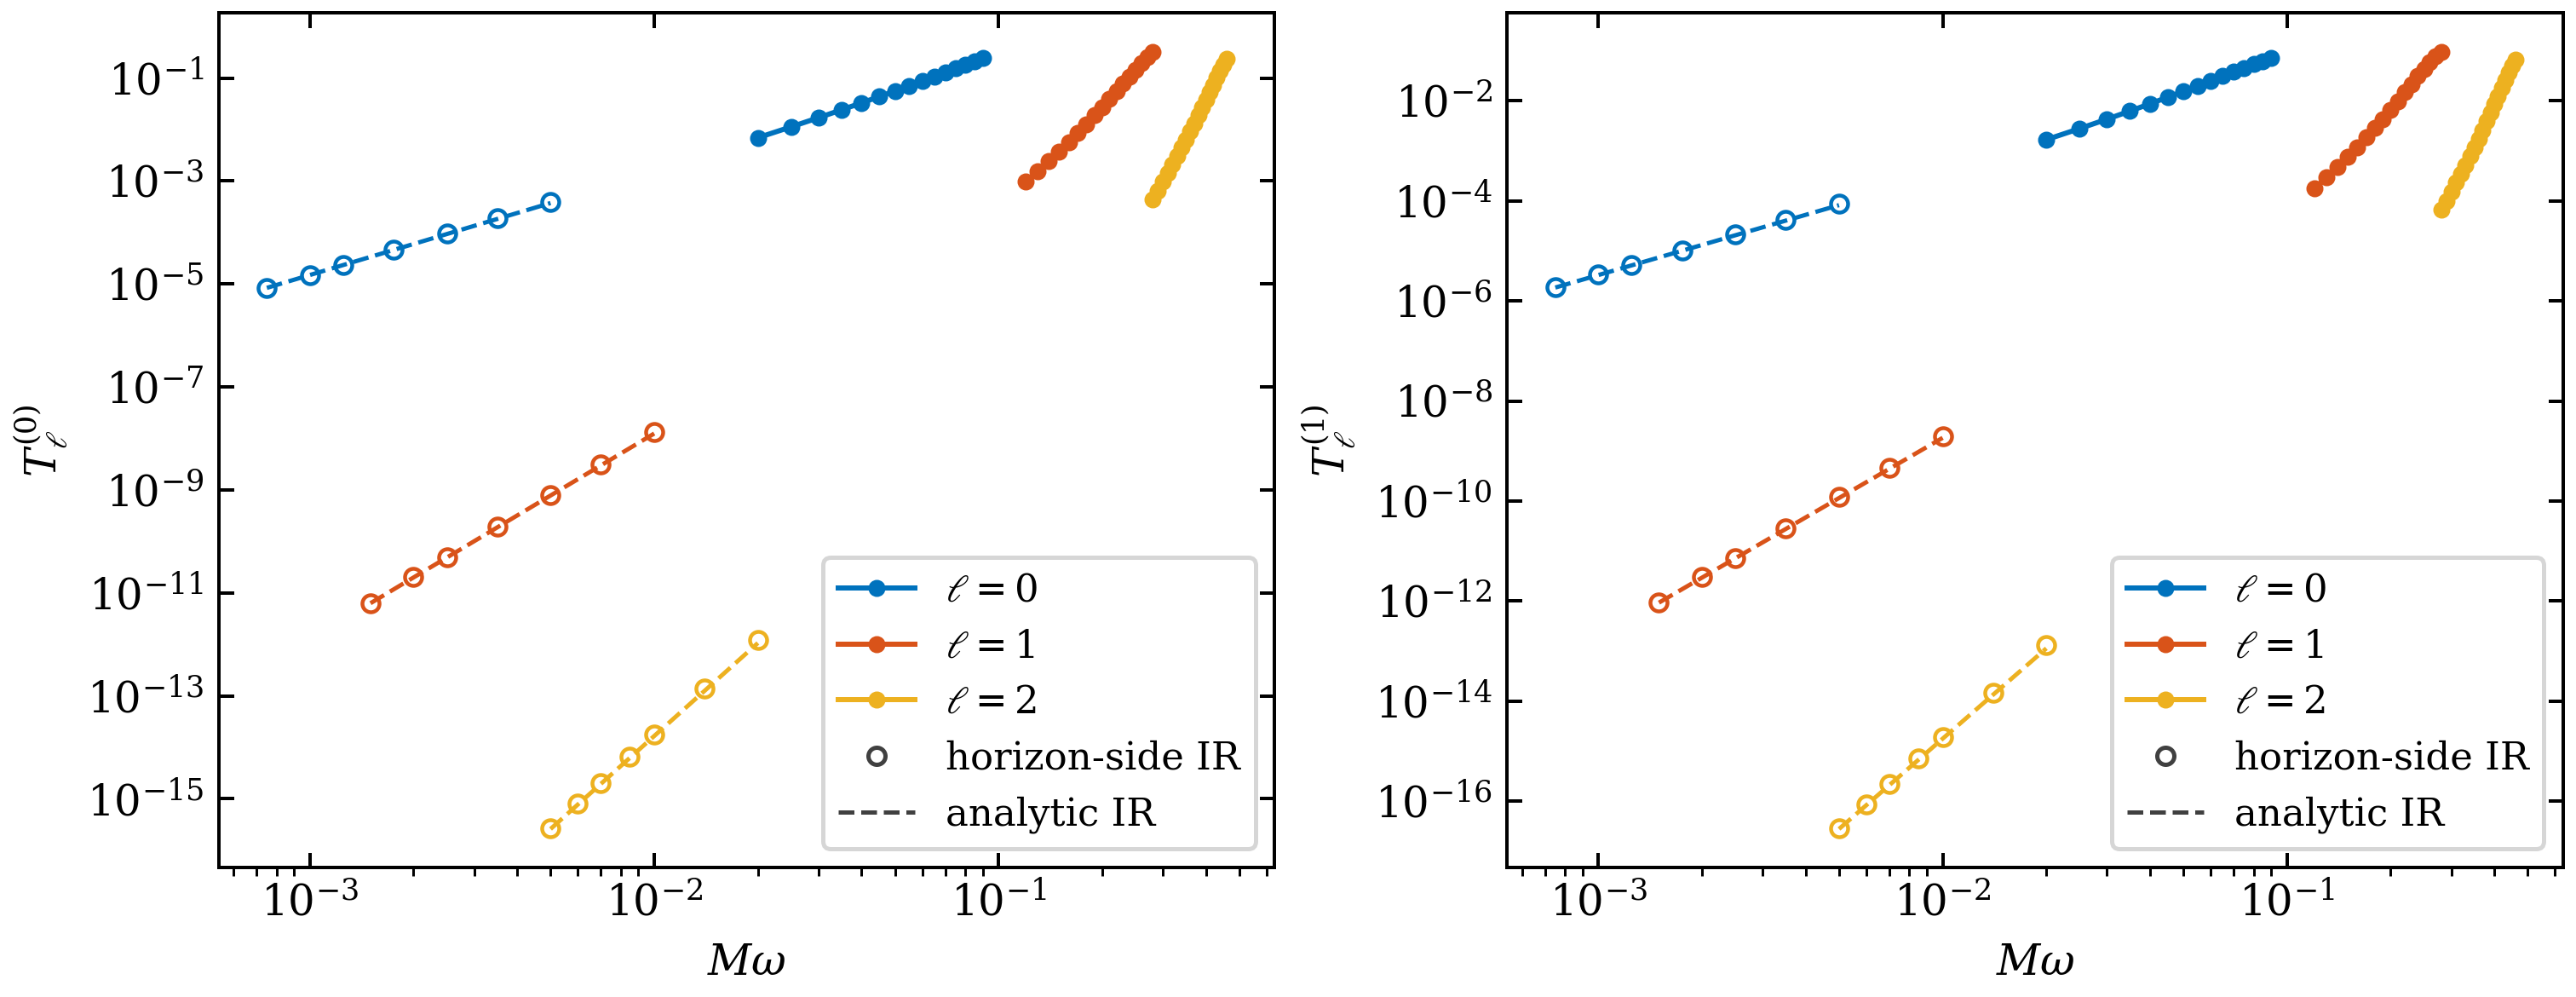
\includegraphics[width=\textwidth]{../../figures/kerr_scalar_low_frequency_axisymmetric.png}
\caption{三次作用的低频吸收。实心点有两端能流共同验证；空心点为更深红外的直接视界侧检查，虚线来自解析领先项。
两类数据之间的空隙标记反射干涉的相消限制，视界响应另有配对收敛检验。}\end{figure}

\subsection{双边能流与视界响应的验证范围}
要求 $|T^{(1)}+R^{(1)}|\le10^{-8}$ 的密集展示低频区间为
$\ell=0:[0.02,0.09]$ 的 15 点，$\ell=1:[0.12,0.28]$ 的 17 点，
$\ell=2:[0.28,0.46]$ 的 19 点。这些区间用于双边能流展示，红外指数由更低频的视界响应和解析式检验。
最低展示点改变谱阶、积分阶、匹配半径后的 $T^{(1)}$ 最大相对变化为 $1.8\times10^{-8}$。
更低频率时，小的反射干涉实部来自大复量的相消，精度下降；$R^{(1)}$ 的独立验证采用该通道的直接投影。
深红外实验只采用直接视界积分、配对加阶、Wronskian 和场残差；其验证等级与双边曲线不同。

\subsection{高次项的明确采点和外推}
$n=2,3$ 的单极计算采用
\begin{align}
M\omega&=(0.0005,0.00075,0.001,0.0015,0.002,0.003,0.005),\\
a/M&=(0,0.5,0.9,0.99,0.999),\qquad (N,q)=(144,144),(176,176).
\end{align}
以最低五点对 $\chi_H^{(n)}/\omega^{2n-2}$ 作二次外推，截距与 $c_n$ 比较。
改用最低四点或六点的截距变化不超过 $4.6\times10^{-6}$。
跨自旋截距相对标准差分别为 $1.2\times10^{-6},7.2\times10^{-7}$。
自由指数范围为 $n=2:2.01009$--$2.01016$，$n=3:4.01552$--$4.01561$，
$R^2>0.9999989$。这里既报告系数，也报告指数和窗口敏感性。

另一组实验沿固定 $y=\omega/\kappa=(0.025,0.05,0.1)$，
$a/M=(0.98,0.99,0.995,0.997,0.999)$ 的路径计算。
在最低 $y$、最高三个自旋上，$\kappa$ 指数为 $2.00734,4.01128$，
$R^2=0.99999988,0.99999993$。
这些数据支持所采路径上的 $\kappa^2,\kappa^4$ 抑制。极端点附近的一致展开需要补充分区误差分析。

\begin{figure}[htbp]\centering
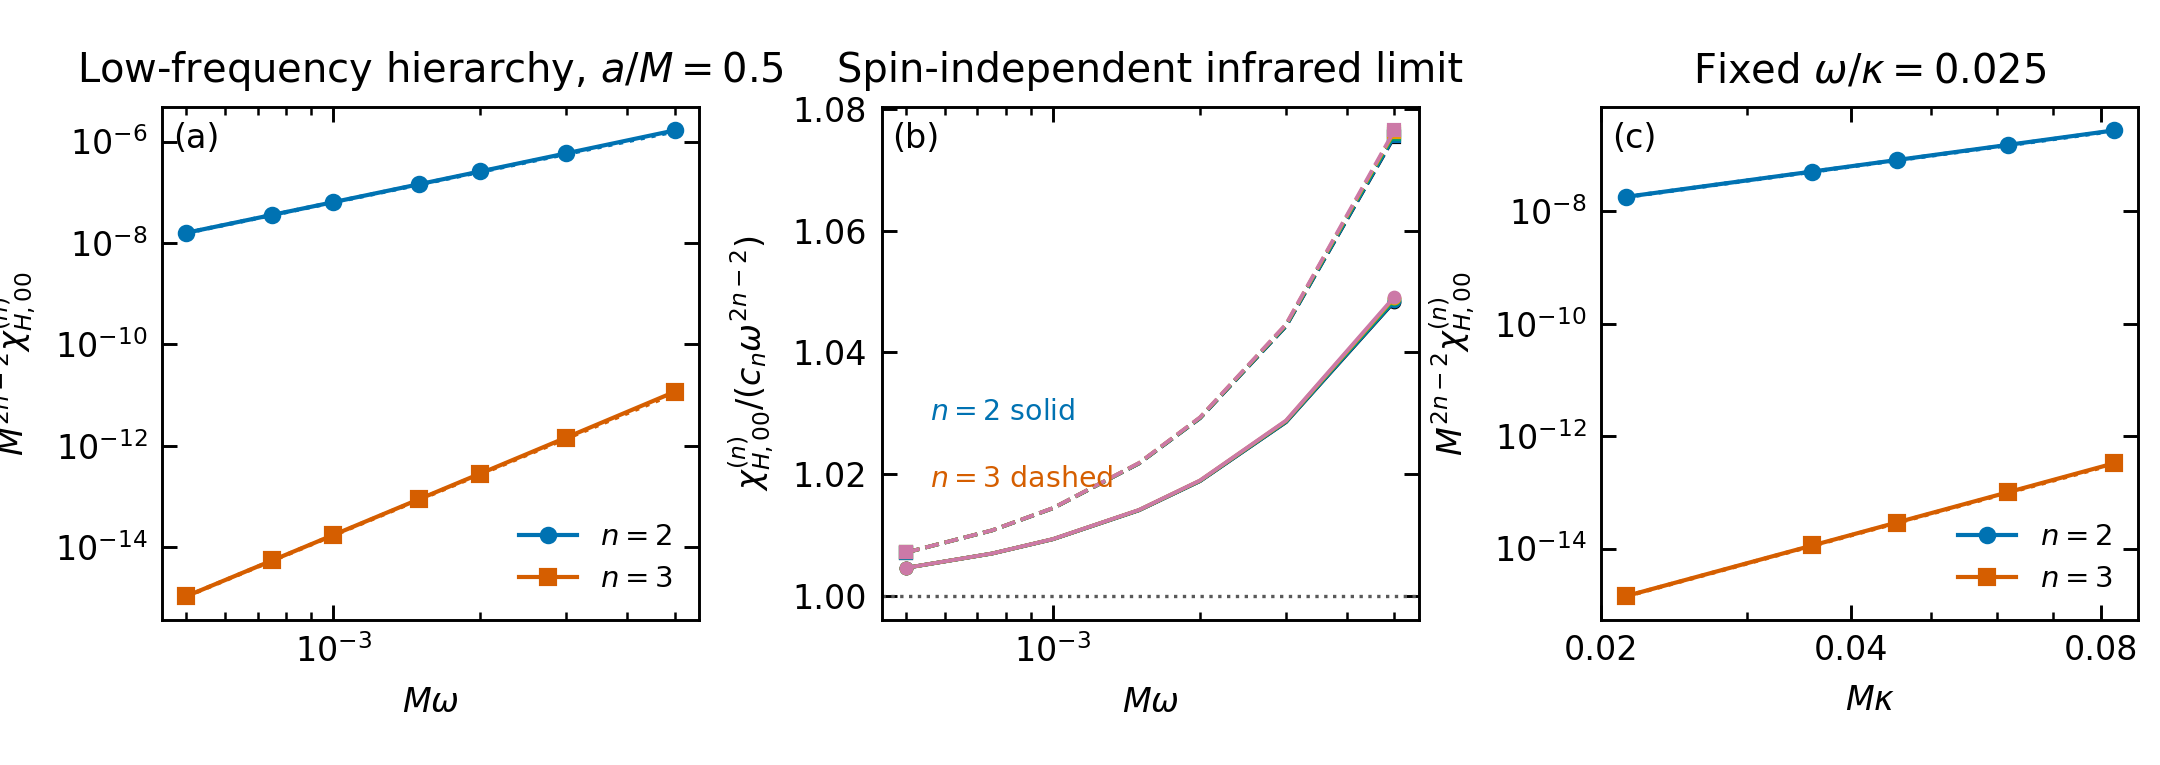
\includegraphics[width=\textwidth]{../../figures/kerr_scalar_power_nonlinearity_l0.png}
\caption{单极高次相互作用。左：相对响应及解析幂次；中：除以领先常数后的跨自旋比较；右：固定 $\omega/\kappa$ 路径。
这里 $m=0$，所以 $p=\omega$；本图检验轴对称单极抑制，principal 增强的证据列于第\ref{sec:principal-v2}节。}\end{figure}

\subsection{有限频率峰与 QNM 频率尺度}
在 $a/M=0.5,m=0$，保留样本的三次 $T^{(1)}$ 均为正。
拟合峰位置为
\begin{equation}M\omega_p=(0.1306,0.3101,0.5026),\end{equation}
相应基本标量 QNM 的实部为 $(0.1124,0.2979,0.4920)$\cite{Berti2009,Stein2019}。
偏移为 $(16.2,4.1,2.2)\%$。拟合形式是
\begin{equation}
T^{(1)}=T_{\rm off}+\frac{A\gamma^2}{(M\omega-\omega_p)^2+\gamma^2},
\quad \gamma=(0.0599,0.0591,0.0595).
\end{equation}
选择高于峰值 $20\%$ 的样本，$R^2=(0.9918,0.9978,0.9985)$，
相对 RMS 残差为 $(2.41,1.27,1.05)\%$。
门槛从 $15\%$ 到 $30\%$ 改变后，峰位置变化不超过
$(6.7,3.9,3.4)\times10^{-4}$，但宽度更敏感。
峰位处于 QNM 频率尺度附近；拟合宽度 $\gamma$ 是所选模型的实频响应参数，QNM 阻尼由复频极点确定。
真正的 QNM 投影要处理复频率、双线性积与轮廓正则化\cite{GreenEtAl2023}。

\begin{figure}[htbp]\centering
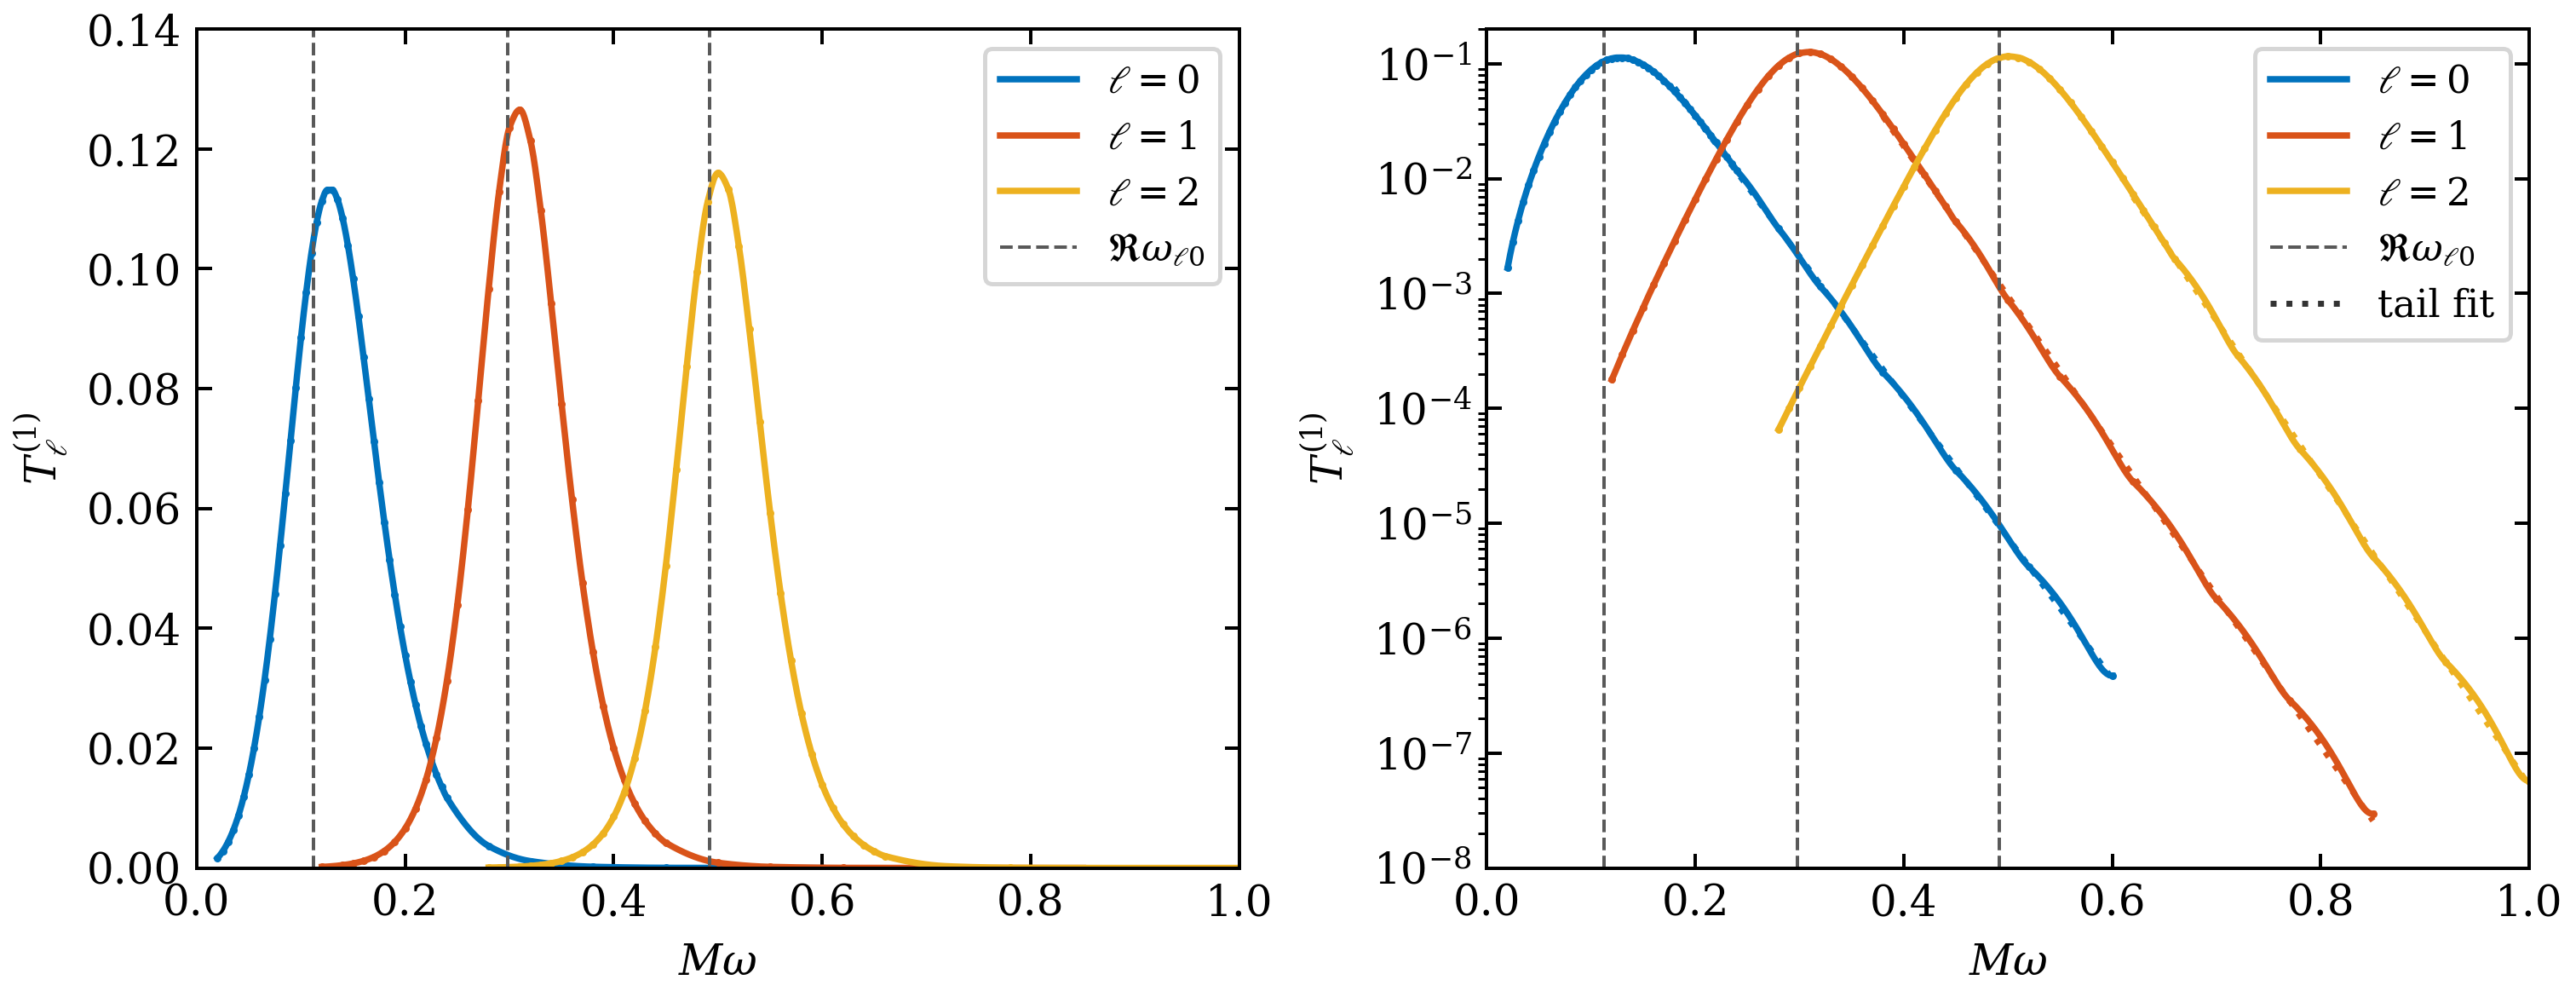
\includegraphics[width=\textwidth]{../../figures/kerr_scalar_nonlinear_axisymmetric_fig2.png}
\caption{有限频率非线性透射。左图显示峰，右图显示有限窗口指数尾；每个圆点是实际保留样本，平滑线仅为保形插值。
虚线标记 QNM 实部；实线为原采样的保形插值。}\end{figure}

\subsection{指数尾：应如何描述“接近热尺度”}
拟合 $\log T^{(1)}=c-\omega/T_{\rm fit}$ 的窗口依次为
$[0.18,0.60],[0.38,0.85],[0.62,1.00]$。
有 19、14、10 个点，合计 43 个，均以 $q=2048$ 重算。
所得 $\pi MT_{\rm fit}=(0.1114,0.1046,0.1012)$，
Kerr Hawking 温度满足
\begin{equation}
T_H=\frac{r_+-r_-}{4\pi(r_+^2+a^2)},\quad\pi MT_H=0.1160\quad(a/M=0.5).
\end{equation}
有效温度偏差为 $4.00\%,9.85\%,12.81\%$。
Hawking 温度\cite{Hawking1975}和灰体因子的有限窗口诊断\cite{Oshita2023,Oshita2024}提供比较尺度；本计算采用经典定态源方程。
与同为两参数的幂律模型比较，指数模型的 $\Delta\mathrm{AICc}$ 优势为 $97.9,48.2,23.8$，
留一预测残差也更小。若强制斜率等于 $-1/T_H$，log RMS 残差增至 $0.139,0.443,0.514$。
所计算窗口的模型比较偏好指数形式，最佳拟合尺度及其与 $T_H$ 的差异由表中数据给出。

\subsection{返回施瓦西的连续性}
固定 $(\ell,m,M\omega)=(2,0,0.52)$，重新计算自旋 $a/M=0,0.05,0.1,0.2,0.3,0.5$。
$T^{(1)}$ 从 $0.0894395$ 平滑增至 $0.103814$，$R^{(1)}$ 为其相反数。
该计算检验端点方程、角投影、源和能流在施瓦西极限的一致性。
\begin{figure}[htbp]\centering
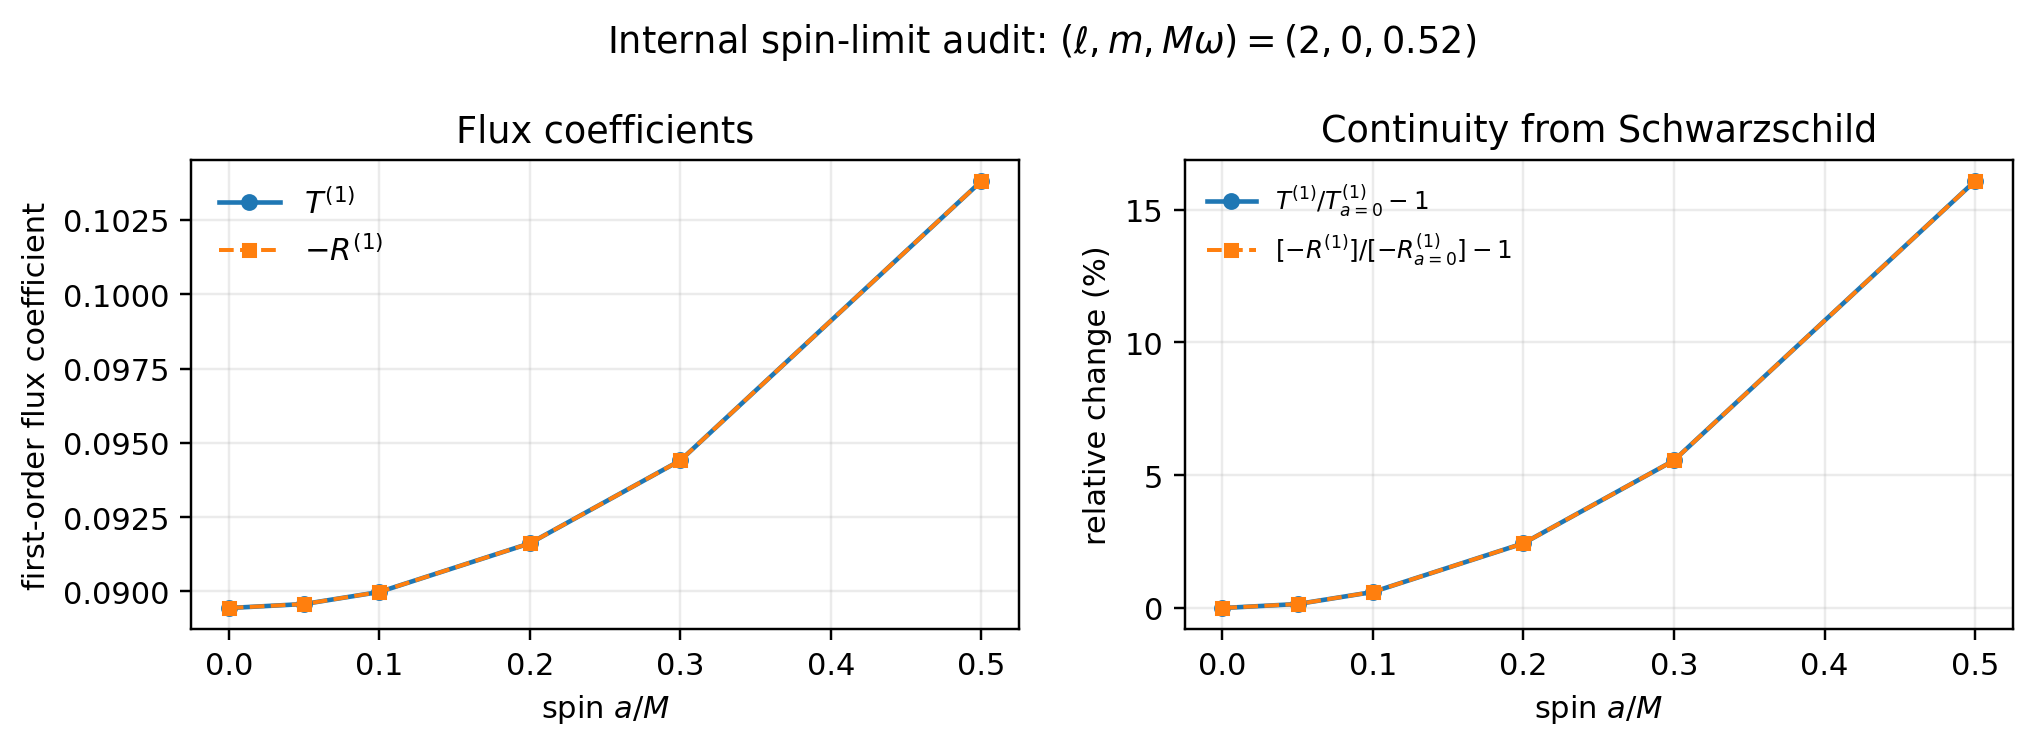
\includegraphics[width=\textwidth]{../../figures/kerr_scalar_spin_limit.png}
\caption{Kerr 到施瓦西的内部连续性检查。转动改变绝对响应；与三次红外分数响应的领先自旋独立性不矛盾，
因为这里频率固定在有限值 $M\omega=0.52$。}\end{figure}

\section{数值可信度：分层误差与独立检验}
\subsection{包含场因子的相对残差}
齐次残差必须定义为
\begin{equation}
\delta_0(r)=\frac{|\Delta R''+\Delta'R'+VR|}
{|\Delta R''|+|\Delta'R'|+|VR|}.
\end{equation}
若分母只包含方程系数，残差会随振幅归一化而改变。
验证采用独立于配点网格的 600 个 Chebyshev--Gauss 点，将谱插值及其导数代入原方程。
谱系数尾定义为最后若干系数的最大模除以全部系数最大模，以保持对场归一化的独立性。

在代表峰点 $a=0.5,\ell=2,m=0,M\omega=0.52$，三支共 1800 个独立点，
残差最大值、95 百分位、中位数为 $2.8\times10^{-10},1.2\times10^{-11},3.2\times10^{-13}$；
最大系数尾 $2.8\times10^{-14}$。
但最低高次单极代表点 $M\omega=5\times10^{-4}$ 的对应数值为
$1.6\times10^{-5},2.1\times10^{-7},2.7\times10^{-10}$。
峰区与红外区具有各自的误差预算和验证参数。

\begin{figure}[htbp]\centering
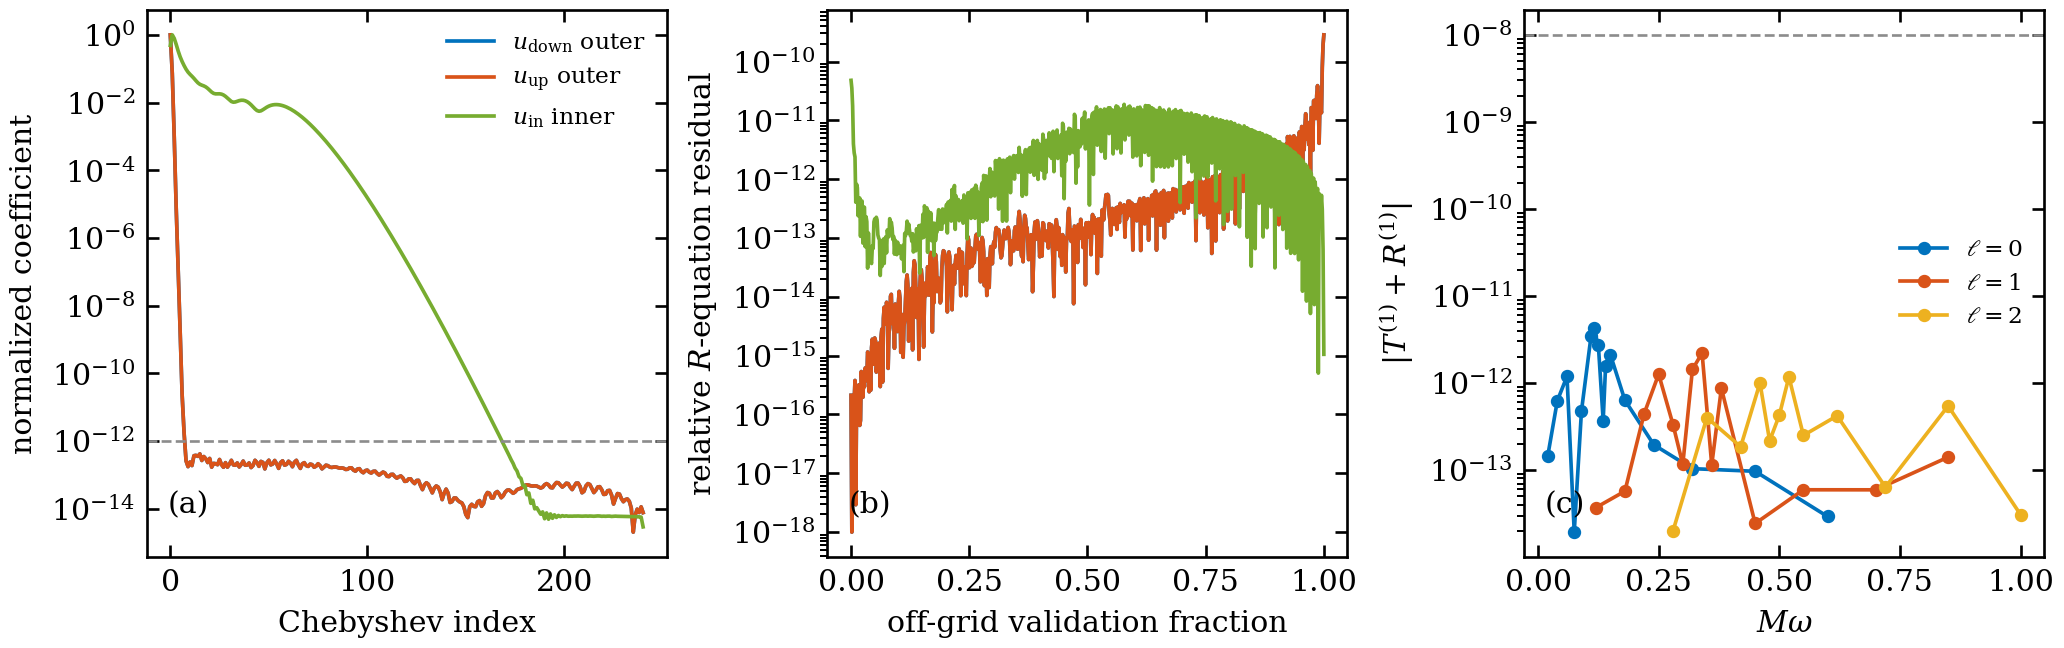
\includegraphics[width=\textwidth]{../../figures/kerr_scalar_axisymmetric_accuracy.png}
\caption{齐次场精度证据：相位剥离后的系数尾、原径向方程的独立点残差、双边能流守恒。
三者分别检验谱截断、局域方程误差和全局守恒。}\end{figure}

\subsection{独立的一阶有源残差}
重构 Green 积分得到 $R_1$ 的节点值，再对它作 Chebyshev 插值和独立求导，检查
\begin{equation}
\delta_{\rm src}=\frac{|\Delta R_1''+\Delta'R_1'+VR_1+Q|}
{|\Delta R_1''|+|\Delta'R_1'|+|VR_1|+|Q|}.
\end{equation}
检验中的二阶导数由场的插值独立求得，以保留方程残差的验证意义。
在 $[3M,8M]$、600 个独立点，重构阶 $D=16,24,32,48,64$。
A、B 是 $a=.5,\ell=m=0,M\omega=.1$ 的 $n=1,2$；
C 是 $a=.99,\ell=m=2,p/\kappa=.5,n=1$ 的局域测试。
在 $D=32$ 处最大残差均低于 $2.3\times10^{-9}$，更高阶出现非单调误差底。
该结果验证所述内区的有源方程。两端积分常数及其余径向区间另需相应检验。

\begin{figure}[htbp]\centering
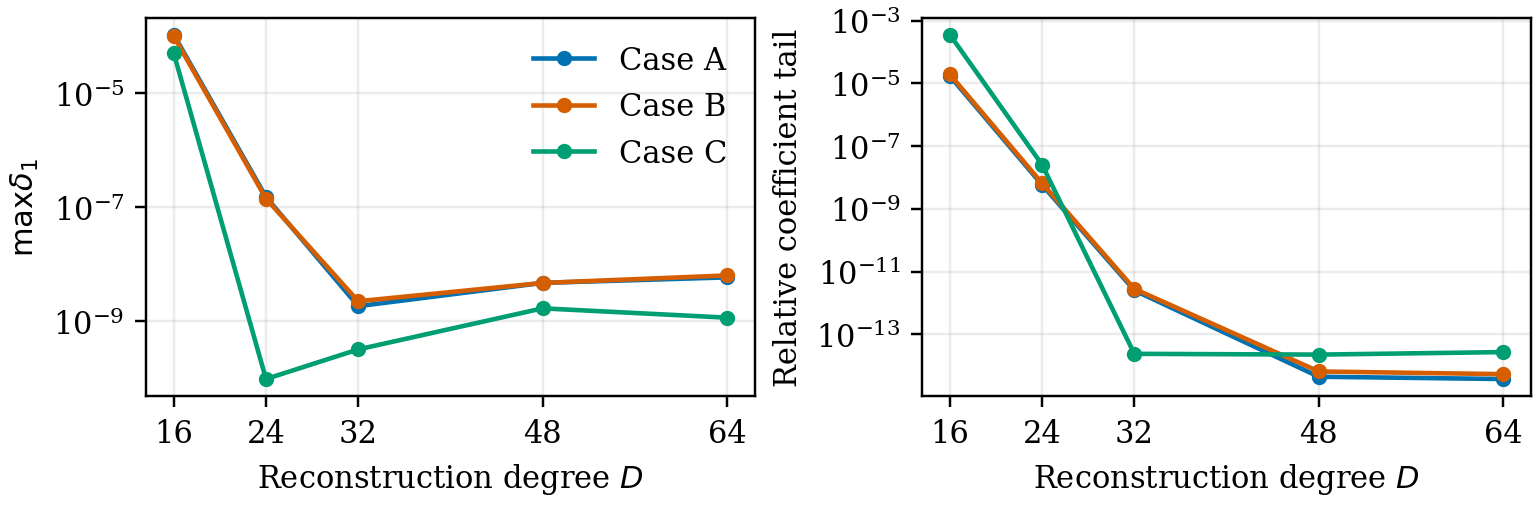
\includegraphics[width=\textwidth]{../../figures/kerr_scalar_sourced_local_validation_20261008.png}
\caption{一阶场的独立局域重构检验。高阶系数尾逐渐减小，二阶导数残差到达非单调误差底限；图中保留全部测试阶数。}\end{figure}

\subsection{误差预算与独立参数扫描}
误差至少分成角基截断、径向谱截断、匹配、积分、浮点相消及拟合模型误差。
角基审计的本征值变化不超过 $4.4\times10^{-16}$，投影不超过 $5.3\times10^{-14}$；这两项低于当前主导误差。
峰区 $(224,160)\to(240,192)$ 的 $T^{(1)}$ 改变最多 $3.1\times10^{-5}$，尽管两端守恒可到 $10^{-12}$。
尾区 $q=1792\to2048$ 的相对变化可到 $2.5\times10^{-4}$，固定积分阶再改变 $N$ 的影响明显更小。
这证明尾区主要受积分而非齐次谱阶限制。

非轴对称探针修正了旧外端行漏掉的 $-2am\omega$，同时使用消去后的稳定系数。
测试 $a/M=.99,.999$、$\ell=m=1,2$、$n=1,2$、$p/\kappa=.5$，
齐次残差最大 $3.2\times10^{-9}$，剥离方程残差最大 $5.2\times10^{-8}$。
错误行对这组响应的变化在 $10^{-8}$ 量级或以下；其证据范围为所列参数，历史全网格需另行复算。
这组检查验证有限参数处的求解器。后文使用另一组近极端数据检验领先解析连接。

\section{Principal 模态与表面引力幂律：解析连接及数值检验}
\label{sec:principal-v2}
\subsection{极限、观测量与证据等级}
本节取实频率、$m>0$、固定非零 $y=p/\kappa$，沿
\begin{equation}
\omega=m\Omega_H+y\kappa,\qquad a/M\longrightarrow1
\end{equation}
研究近极端响应。这条路径的频率趋向 $m/(2M)$。
它与前文固定自旋的 $\omega\to0$ 红外极限具有不同的主导区域。
非线性展开仍为 $\Box\Phi+\epsilon_n|\Phi|^{2n}\Phi=0$，
观测量为固定入射的自通道系数
\begin{equation}
\widehat\chi_n\equiv M^{2n-2}\frac{T_n^{(1)}}{T^{(0)}}
=M^{2n-2}\frac{2\Rea A_{H,n}^{(1)}}{|\Bin|^{2n}}.
\label{eq:principal-observable-v2}
\end{equation}
近区超几何解与外区连接是线性解析工具\cite{BredbergKerrCFT2010,MST1996}。
本节将这些解代入本项目的非线性源积分，明确列出领先包络的成立条件。
采用的计算实现为近极端首阶超几何--Whittaker 匹配；完整 MST 级数提供进一步求取次领先项的路线。
下面先取 $M=1$ 完成连接与积分，最后恢复无量纲观测量。

\subsection{从径向方程得到喉部算符与共形权重}
定义
\begin{equation}
\sigma=\frac{r_+-r_-}{M},\qquad
X=\frac{r-r_+}{r_+-r_-},\qquad
M\kappa=\frac{\sigma}{4(1+\sigma/2)}.
\end{equation}
因此 $\sigma\sim4M\kappa$。在 $M=1$ 的变量中，
\begin{equation}
\Delta=\sigma^2X(X+1),\qquad
K=\sigma\left(\frac y2+2r_+\omega X+\omega\sigma X^2\right).
\end{equation}
这里用到了 $(r_+^2+a^2)p=(r_+-r_-)y/2$。固定 $X$ 取 $\sigma\to0$，得到
\begin{equation}
\mathcal L_y f\equiv
\frac{\dd}{\dd X}\left[X(X+1)\frac{\dd f}{\dd X}\right]
+\left[\frac{(mX+y/2)^2}{X(X+1)}-\lambda_\star\right]f=0,
\label{eq:near-operator-v2}
\end{equation}
其中 $A_\star=A_{\ell m}(m/2)$、$\lambda_\star=A_\star-3m^2/4$。
在 $X\gg1$ 的重叠区，设 $f\sim X^q$，指标方程为
\begin{equation}
q(q+1)+m^2-\lambda_\star=0,
\qquad
h=\frac12+\sqrt{\frac14+A_\star-\frac{7m^2}{4}}.
\end{equation}
两条支解的幂次为 $h-1$ 和 $-h$。
负的根号判别式定义 principal 模态，此时 $h=1/2+\ii\beta$、$\beta>0$。
正判别式给出实权重 supplementary 模态；零判别式属于需要对数支解的临界情形。
喉部权重 $h$ 描述本极限的指标，MST 重整化角动量 $\nu$ 则用于完整径向级数的连接。

\subsection{近区超几何解及两个连接系数}
满足视界入射条件的领先解为
\begin{equation}
\begin{split}
f_y(X)={}&X^{-\ii y/2}(1+X)^{\ii(y/2-m)}\\
&\times{}_2F_1(h-\ii m,1-h-\ii m;1-\ii y;-X).
\end{split}
\label{eq:near-f-v2}
\end{equation}
原点处 $f_y\sim X^{-\ii y/2}$，因此其入射振幅为一。
超几何连接公式给出
\begin{equation}
f_y\sim c_+X^{h-1}+c_-X^{-h},
\end{equation}
\begin{align}
c_+&=\frac{\Gamma(1-\ii y)\Gamma(2h-1)}
{\Gamma(h-\ii m)\Gamma(h-\ii(y-m))},\\
c_-&=\frac{\Gamma(1-\ii y)\Gamma(1-2h)}
{\Gamma(1-h-\ii m)\Gamma(1-h-\ii(y-m))}.
\end{align}
对 principal 模态，两支的模均按 $X^{-1/2}$ 衰减，两个连接系数在领先阶共同参与匹配。
径向流守恒给出独立恒等式
\begin{equation}
\beta(|c_+|^2-|c_-|^2)=-\frac y2.
\label{eq:near-current-v2}
\end{equation}

\subsection{外区 Whittaker 解与固定入射增强}
极端临界频率处，设 $u=r-1$、$\psi=uR$，外区方程化为
\begin{equation}
\psi''+\left[\frac{m^2}{4}+\frac{m^2}{u}
+\frac{m^2-\lambda_\star}{u^2}\right]\psi=0.
\end{equation}
取 $z=-\ii mu$，这是参数 $(\ii m,h-1/2)$ 的 Whittaker 方程。
以重叠区幂次为归一化的两支可写成
\begin{equation}
\mathcal R_+=\frac{(-\ii m)^{-h}}u M_{\ii m,h-1/2}(-\ii mu),\qquad
\mathcal R_- =\frac{(-\ii m)^{h-1}}u M_{\ii m,1/2-h}(-\ii mu).
\end{equation}
分别满足 $\mathcal R_+\sim u^{h-1}$、$\mathcal R_-\sim u^{-h}$。
采用主值复幂，其无穷远入射系数为
\begin{align}
U_+&=\frac{\Gamma(2h)}{\Gamma(h-\ii m)}(-\ii m)^{-h-\ii m},\\
U_-&=\frac{\Gamma(2-2h)}{\Gamma(1-h-\ii m)}(-\ii m)^{h-1-\ii m}.
\end{align}
共同的单位模相位由龟坐标常数决定，在能流与相对响应中约去。
匹配 $u\sim\sigma X$ 后，单位视界解的入射系数为
\begin{equation}
\Bin\sim c_+U_+\sigma^{1-h}+c_-U_-\sigma^h
=\sigma^{1/2}D(\theta),\qquad \theta=\beta\ln\sigma,
\end{equation}
\begin{equation}
D(\theta)=c_+U_+e^{-\ii\theta}+c_-U_-e^{\ii\theta}.
\label{eq:principal-D-v2}
\end{equation}
固定入射解 $R_0=R_{\rm in}/\Bin$ 因而满足
\begin{equation}
|R_0(X)|^2\sim\sigma^{-1}\frac{|f_y(X)|^2}{|D(\theta)|^2}.
\end{equation}
这给出 principal 模态的场强增强。视界能流还含有 $p\propto\sigma$，两项相乘得到有限的领先吸收：
\begin{equation}
T^{(0)}\sim\frac{y}{m|D(\theta)|^2}.
\end{equation}

\subsection{Green 积分的收敛性与非线性阶次}
记纯出射外区解的重叠区系数为
\begin{align}
g_+&=\frac{\Gamma(1-2h)}{\Gamma(1-h-\ii m)}(-\ii m)^h,\\
g_-&=\frac{\Gamma(2h-1)}{\Gamma(h-\ii m)}(-\ii m)^{1-h}.
\end{align}
取喉部两支 $\varphi_+\sim X^{h-1}$、$\varphi_-\sim X^{-h}$，定义
\begin{equation}
v_\theta=g_+e^{\ii\theta}\varphi_++g_-e^{-\ii\theta}\varphi_-,\qquad
R_{\rm up}\sim\sigma^{-1/2}v_\theta.
\end{equation}
物理 Wronskian 满足
\begin{equation}
W=\Delta(R_{\rm in}R_{\rm up}'-R_{\rm up}R_{\rm in}')
\sim\sigma^{1/2}w_\theta,\qquad
w_\theta=X(X+1)(f_yv_\theta'-v_\theta f_y').
\end{equation}
于是 $R_{\rm up}\dd r/W\sim v_\theta\dd X/w_\theta$。
这一步明确消去了径向积分测度与 Green 核中的表面引力因子。
定义临界频率处的实角投影 $\mathcal C_n=C_{\ell\ell m}^{(0,n)}+C_{\ell\ell m}^{(2,n)}$，单位视界源给出
\begin{equation}
\mathcal A_n(\theta,y)
=-\frac{\mathcal C_n}{w_\theta}\int_0^\infty
v_\theta |f_y|^{2n}f_y\,\dd X.
\label{eq:principal-A-v2}
\end{equation}
对 principal 支解，积分上端的包络为 $X^{-n-1}$；原点的模有界。
因此每个正整数 $n$ 的领先积分绝对收敛。重叠区外端的尾项与外区场通过匹配进入次领先贡献。
在固定非零 $y$、$D$ 与 $w_\theta$ 保持非退化的参数范围内，
\begin{equation}
\boxed{\widehat\chi_n
=\sigma^{-n}\mathcal F_n(y,\theta)+o(\sigma^{-n}),\qquad
\mathcal F_n=\frac{2\Rea\mathcal A_n}{|D|^{2n}}.}
\label{eq:principal-envelope-v2}
\end{equation}
恢复 $\sigma\sim4M\kappa$ 后，这就是带有界相位调制的 $(M\kappa)^{-n}$ 包络。
三次项 $n=1$ 给出 $\kappa^{-1}$，五次项 $n=2$ 给出 $\kappa^{-2}$。
若某个参数点的 $\Rea\mathcal A_n=0$，该点的响应由次领先项决定。

\subsection{可直接计算的解析系数与对数周期}
为对应已有脚本，令 $d=|c_+|^2-|c_-|^2$，$\gamma_+=g_+e^{\ii\theta}$、$\gamma_-=g_-e^{-\ii\theta}$。
principal 情形下，$f_y^*$ 的两支系数交换并取共轭，因此
\begin{align}
v_\theta&=\alpha_\theta f_y+b_\theta f_y^*,\\
\alpha_\theta&=(\gamma_+c_+^*-\gamma_-c_-^*)/d,\qquad
b_\theta=(-\gamma_+c_-+\gamma_-c_+)/d,\\
w_\theta&=\ii y b_\theta.
\end{align}
定义两个收敛积分
\begin{equation}
I_{{\rm osc},n}=\int_0^\infty f_y^2|f_y|^{2n}\dd X,\qquad
I_{{\rm abs},n}=\int_0^\infty|f_y|^{2n+2}\dd X,
\end{equation}
则
\begin{equation}
\mathcal A_n=\frac{\ii\mathcal C_n}{y}
\left(\frac{\alpha_\theta}{b_\theta}I_{{\rm osc},n}+I_{{\rm abs},n}\right).
\label{eq:principal-computable-v2}
\end{equation}
这给出零拟合参数的领先预测；其特殊函数连接系数为解析表达，源积分通过独立求积求值。
在领先式中，$\theta\mapsto\theta+\pi$ 使 $D$ 和 $v_\theta$ 同时变号，故 $\mathcal F_n$ 的周期为 $\pi$。
对应的 $\ln\sigma$ 周期为 $\pi/\beta$。在 $\mathcal F_n\ne0$ 的区间，局部有效斜率为
\begin{equation}
\frac{\dd\ln|\widehat\chi_n|}{\dd\ln(M\kappa)}
=-n+\frac{\dd\ln|\mathcal F_n|}{\dd\ln(M\kappa)}+o(1).
\end{equation}
因此实部 $\Rea h=1/2$ 决定包络，虚部 $\beta$ 决定对数相位。

\subsection{Supplementary 模态的区域贡献}
对一般实权重 $h>1/2$，主连接给出 $R_0\sim\sigma^{h-1}f_y$。
使用喉部向外衰减支解时，源积分上端的幂次为
\begin{equation}
X^{-h}|X^{h-1}|^{2n}X^{h-1}
=X^{2n(h-1)-1}.
\end{equation}
这确定了分区积分的三种情况：$1/2<h<1$ 的喉部上端收敛，候选领先因子为 $\sigma^{2n(h-1)}$；
$h=1$ 的上端积分产生对数，需要采用相应的退化连接；$h>1$ 的积分依赖 $X\sim\sigma^{-1}$ 的匹配上限。
在 $h>1$ 情形，该上限贡献提供 $\sigma^{-2n(h-1)}$，与固定入射因子相乘得到零次幂量级，首项系数由完整外区匹配决定。
这些是区域计数及其收敛条件，实权重通道的完整首项仍需逐模求取。
临界频率处，本项目的角本征值给出 $h_{11}=1.1706059743$、$h_{22}=1/2+0.9459584692\ii$。
这解释了为何 $(1,1)$ 控制通道需要保留外区贡献，而 $(2,2)$ 具有收敛的 principal 喉部积分。

\subsection{已有数值对领先解析式的检验}
2026 年 10 月 13 日的数据取 $y=0.5$、$\ell=m=1,2$、$n=1,2$，
在 $a/M=0.99,0.999,0.9999,0.99999,0.999999$ 上比较 $(N,q)=(256,1024)$ 与 $(320,1536)$。
principal 响应的最大配对相对变化为 $1.29\times10^{-5}$。
进一步的 $(384,2048)$、$(448,3072)$ 检查覆盖 $a/M=0.999999,0.9999999$，分别记录视界响应和双边能流质量门槛。
计算记录的进程工作集约为 $74$--$79$ MB。
下表展示 $N=320$、通过 $|T_n^{(1)}+R_n^{(1)}|\le10^{-8}$ 的代表点。
\begin{table}[htbp]\centering\small
\caption{Principal $(2,2)$ 自通道：完整 Kerr 计算与零拟合参数的领先匹配预测。固定 $y=0.5$。}
\begin{tabular}{ccrrr}\toprule
$a/M$ & $n$ & $\chi_H^{(n)}$（谱解） & $\chi_H^{(n)}$（首阶匹配） & 相对差异\\\midrule
0.99999 & 1 & 23.910575 & 24.530074 & $2.591\%$\\
0.999999 & 1 & 76.277602 & 76.906770 & $0.825\%$\\
0.99999 & 2 & 194.125279 & 199.588366 & $2.814\%$\\
0.999999 & 2 & 1967.775232 & 1986.739546 & $0.964\%$\\\bottomrule
\end{tabular}\end{table}
首阶匹配差异包含有限 $\sigma$ 的次领先修正；其量级大于所列点的配对分辨率变化。
数据支持 $(2,2)$ 的 $n=1,2$ 领先包络与系数表达，向其他 principal 模态及一般 $y$ 的检验列入后续计算。
角本征值 $A_{22}(1)=5.855162574589$，角源系数 $\mathcal C_1=0.122592732894$、$\mathcal C_2=0.0147336525753$。
解析近区方程在 $X=0.1,1,10$ 以 32 位十进制运算检查，相对残差低于 $8\times10^{-34}$。
源积分采用 $t=\ln X\in[-36,36]$，每个单位子区间比较 12 与 20 阶 Gauss 求积；配对变化低于 $6\times10^{-16}$。
这项比较检验固定截取区间的求积稳定性，完整误差还包含尾区截取和连接近似。
对 $a/M=0.999999$ 的 $N=320$ 齐次谱解，600 个离网点的径向最大相对残差为 $3.2\times10^{-9}$，剥相位残差为 $7.3\times10^{-8}$。
更极端的 $a/M=0.9999999$ 数据保留在诊断文件中，并以各自的双边门槛标记区分展示等级。

\subsection{微扰控制参数与物理含义}
令 $\widehat\epsilon_n=\epsilon_n/M^{2n-2}$，固定入射振幅为 $\mathcal A_{\rm in}$。
principal 扇区的领先相对修正为
\begin{equation}
\frac{T-T^{(0)}}{T^{(0)}}
\sim\widehat\epsilon_n|\mathcal A_{\rm in}|^{2n}
(M\kappa)^{-n}\widetilde{\mathcal F}_n.
\end{equation}
微扰有效域要求该量的模及复振幅修正同时远小于一。
在调制函数保持有限非零的参数区间，有效小参数随 $\kappa^{-n}$ 增大；提高相互作用阶次会加强这种近极端敏感性。
这里建立的是固定背景、首阶定态响应的包络与系数路线。
非线性饱和、时间演化和反作用需要有限耦合或时间域计算。

\section{把结果放回完整物理图景}
\subsection{新的信息是什么}
第一，绝对吸收趋向零时，三次项保留有限的红外分数响应。
第二，领先分数系数的自旋独立性来自近区归一化因子的抵消，有明确的解析机制和适用域。
第三，单极高次相互作用形成可解析的阶数层级，$2n-2$ 表示固定自旋红外相对响应的指数。
第四，复响应包含不在能流实部中的相位信息，单极的 $\ii/4$ 是独立的领先预测。
第五，有限频率旋转连续性与红外自旋独立性相容：二者对应不同的观测量与极限。
第六，principal 近极端自通道具有另一条阶数层级：在非退化连接和收敛源积分条件下，相对响应包络按 $\kappa^{-n}$ 增强。
其来源是固定入射场强的 $\kappa^{-1}$ 增强；复权重虚部引入可计算的对数相位调制。

\subsection{最终结论的合格表述}
在固定亚极端 Kerr 背景上，弱 $U(1)$ 对称标量自相互作用的首阶定态吸收可以由端点包含的谱解和协变 Green 积分求得。
对三次轴对称自通道，匹配渐近证明线性和首阶吸收具有相同的 $(M\omega)^{2\ell+2}$ 红外指数；
两者之比及相对相位趋向由远区球 Bessel 积分决定的、自旋独立的常数。
单极更一般的 $|\Phi|^{2n}\Phi$ 相互作用具有正的解析系数和 $(M\omega)^{2n-2}$ 分数响应层级，
并已有 $n=2,3$ 多自旋数值实验支持。
近极端 principal 自通道的领先匹配给出带相位调制的 $\kappa^{-n}$ 包络，已有 $(2,2)$、$y=0.5$、$n=1,2$ 的独立谱解支持。
有限频率的峰和指数尾提供窗口内的现象学结果；QNM 极点和热谱的判定各需对应的谱分析与物理假设。
所有结论保留耦合符号、振幅归一化、验证等级和极限次序。

\subsection{仍需要完成的工作}
完整模式耦合一阶场与二阶能流；近极端次领先项、一般 $y$ 与其他模态的连接检验；覆盖整个径向域的有源残差；
时间域扰动有效性与非线性饱和；外部独立求解器检查；稳定的公开数据与代码版本归档。
计算精度按局域误差、积分误差、连接近似与拟合误差分别报告。

\section{复习顺序与可复核记录}
建议依次独立复算：施瓦西 $u/r$ 重定义；Kerr 算符分离；能流正负号；
Green 导数跳跃；$|\alpha|^{2n}\alpha$ 的归一化；$I_0,J_0$；Legendre--Bessel 匹配；
全 $n$ 积分正性；最后才读数值曲线。若其中一个归一化不清楚，应暂停比较任何拟合指数。

本笔记对应主稿位于 \nolinkurl{docs/prd/kerr_scalar_nonlinear_prd_review_20261007.tex}，
验证记录为 \nolinkurl{docs/prd/PRD_VALIDATION_20261008.md}。
新增近极端解析实现为 \nolinkurl{scripts/analyze_principal_matching_20261013.py}，
匹配结果为 \nolinkurl{results/kerr_scalar_principal_matched_prediction_20261013.csv}，
连接与求积检查为 \nolinkurl{results/kerr_scalar_principal_matching_checks_20261013.json}。
本次更新引用上述既有记录，新增范围为笔记文字与编译输出。
有源检验数据为 \nolinkurl{results/kerr_scalar_sourced_local_residual_20261008.csv}。
下述附录从该主稿原表机械提取数值，不新增或平滑数据；表头保留原符号以便逐项对应。
文献表也沿用主稿书目信息，未将其标记为本次重新联网核查的结果。
\clearpage\appendix
\section{完整数值表与审计数据}
\begin{table}[htbp]
\centering
\caption{角向离散审计：本征值和两个源投影相对于额外 24 个基与 512 点参考配置的最大相对变化。}
\label{note-tab:angular-convergence}
\begin{adjustbox}{max width=\textwidth}
\begin{tabular}{lccc}
setting $(L_{\rm extra},q_\theta)$ & $\max\Delta\lambda$
& $\max\Delta C^{(0)}$ & $\max\Delta C^{(2)}$\\
\midrule
active $(16,256)$ & $4.4\times10^{-16}$ & $3.7\times10^{-14}$ & $5.2\times10^{-14}$\\
basis $(12,512)$ & $4.4\times10^{-16}$ & $1.6\times10^{-16}$ & $0$\\
quadrature $(24,128)$ & $0$ & $1.5\times10^{-14}$ & $2.0\times10^{-14}$\\
\end{tabular}
\end{adjustbox}
\end{table}

\begin{table}[htbp]
\centering
\caption{三次轴对称红外解析系数及直接视界侧检验，$a/M=0.5$。最后一列比较两组谱阶和积分阶。}
\label{note-tab:axisymmetric-infrared}
\begin{adjustbox}{max width=\textwidth}
\begin{tabular}{c c c c c c c}
$\ell$ & ${\cal I}_\ell$ & $\chi^{\rm IR}_\ell$
& ${\cal A}^{(0)}_\ell$ & ${\cal A}^{(1)}_\ell$
& lowest $M\omega$ & $\delta_N\chi_H$\\
\hline
0 & 0.346573590280 & 0.220635600153 & 14.9282032 & 3.29369308 & 0.00075 & $1.1\times10^{-7}$\\
1 & 0.128401008797 & 0.147136717786 & 1.24401694 & 0.183040569 & 0.00150 & $1.5\times10^{-4}$\\
2 & 0.077970747421 & 0.106366541731 & 0.0165868925 & 0.00176429039 & 0.00500 & $7.7\times10^{-5}$\\
\end{tabular}
\end{adjustbox}
\end{table}

\begin{table}[htbp]
\centering
\caption{通过双边首阶能流门槛的低频展示区间、点数和最低点的实际结果。}
\label{note-tab:low-acceptance}
\begin{adjustbox}{max width=\textwidth}
\begin{tabular}{c c c c c c}
$\ell$ & displayed $M\omega$ range & points
& $T^{(0)}_{\rm low}$ & $T^{(1)}_{\rm low}$ & $|\delta_1|_{\rm low}$\\
\hline
0 & $[0.02,0.09]$ & 15 & $6.92348\times10^{-3}$ & $1.67885\times10^{-3}$ & $1.4\times10^{-13}$\\
1 & $[0.12,0.28]$ & 17 & $9.73095\times10^{-4}$ & $1.78519\times10^{-4}$ & $3.7\times10^{-14}$\\
2 & $[0.28,0.46]$ & 19 & $4.35440\times10^{-4}$ & $6.58814\times10^{-5}$ & $2.0\times10^{-14}$\\
\end{tabular}
\end{adjustbox}
\end{table}

\begin{table}[htbp]
\centering
\caption{各多极最低展示点的独立参数审计：改变谱阶、积分阶或匹配半径，相对参考 $(256,256,40)$ 比较。}
\label{note-tab:low-convergence}
\begin{adjustbox}{max width=\textwidth}
\begin{tabular}{c c c c c c}
$\ell$ & $M\omega$ & $T^{(1)}_{\rm ref}$
& $\max|\Delta T^{(1)}/T^{(1)}|$
& $\max|\Delta R^{(1)}/R^{(1)}|$ & $\max|\delta_1|$\\
\hline
0 & 0.02 & $1.67885\times10^{-3}$ & $1.8\times10^{-8}$ & $2.0\times10^{-8}$ & $3.0\times10^{-12}$\\
1 & 0.12 & $1.78519\times10^{-4}$ & $6.7\times10^{-9}$ & $7.3\times10^{-9}$ & $3.8\times10^{-13}$\\
2 & 0.28 & $6.58814\times10^{-5}$ & $9.2\times10^{-9}$ & $4.6\times10^{-9}$ & $2.8\times10^{-13}$\\
\end{tabular}
\end{adjustbox}
\end{table}

\begin{table}[htbp]
\centering
\caption{单极高次作用的解析常数、拟合指数、外推系数误差与双分辨率变化；固定 $y$ 为 $y=0.025$。}
\label{note-tab:power-l0}
\begin{adjustbox}{max width=\textwidth}
\begin{tabular}{c c c c c c c}
$n$ & $c_n$ & predicted power & fixed-$\omega$ fitted power
& fixed-$y$ $\kappa$ power & max. coefficient error & max. $\delta_N\chi_H$\\
\hline
2 & 0.0631722552 & 2 & 2.01009--2.01016 & 2.00734 & $2.8\times10^{-6}$ & $2.5\times10^{-6}$\\
3 & 0.0172436384 & 4 & 4.01552--4.01561 & 4.01128 & $1.3\times10^{-6}$ & $7.7\times10^{-9}$\\
\end{tabular}
\end{adjustbox}
\end{table}

\begin{table}[htbp]
\centering
\caption{有限频率峰和指数尾的现象学拟合参数。QNM 为基本标量模，频率单位 $M=1$；$\Delta T$ 是与 Hawking 温度的相对偏差。}
\label{note-tab:fit}
\begin{adjustbox}{max width=\textwidth}
\begin{tabular}{c c c c c c c}
$\ell$ & $\omega_p$ & $\gamma$
& $\Re\omega_Q$
& $|\Im\omega_Q|$
& $\pi T_{\rm fit}$
& $\Delta T$\\
\hline
0 & 0.1306 & 0.0599 & 0.1124 & 0.1022 & 0.1114 & 4.00\%\\
1 & 0.3101 & 0.0591 & 0.2979 & 0.0954 & 0.1046 & 9.85\%\\
2 & 0.5026 & 0.0595 & 0.4920 & 0.0946 & 0.1012 & 12.81\%\\
\end{tabular}
\end{adjustbox}
\end{table}

\begin{table}[htbp]
\centering
\caption{移动指数尾拟合窗口后的有效温度范围、log 残差与温度偏差；不是无限高频误差界。}
\label{note-tab:tail-window}
\begin{adjustbox}{max width=\textwidth}
\begin{tabular}{c c c c c c}
$\ell$ & baseline $[M\omega_{\min},M\omega_{\max}]$
& $\pi T_{\rm fit}^{\rm base}$ & range of $\pi T_{\rm fit}$
& $\max\sigma_{\log}$ & $\max|T_{\rm fit}/T_H-1|$\\
\hline
0 & $[0.18,0.60]$ & 0.1114 & $[0.1109,0.1122]$ & $3.86\times10^{-2}$ & 4.45\%\\
1 & $[0.38,0.85]$ & 0.1046 & $[0.1037,0.1068]$ & $6.95\times10^{-2}$ & 10.61\%\\
2 & $[0.62,1.00]$ & 0.1012 & $[0.1002,0.1031]$ & $5.59\times10^{-2}$ & 13.62\%\\
\end{tabular}
\end{adjustbox}
\end{table}

\begin{table}[htbp]
\centering
\caption{指数与幂律尾的同参数数目比较。正的 $\Delta\mathrm{AICc}$ 支持指数模型，LOO 为留一预测误差。}
\label{note-tab:tail-models}
\begin{adjustbox}{max width=\textwidth}
\begin{tabular}{c c c c c c c}
$\ell$ & points & $\sigma_{\rm exp}$ & $\sigma_{\rm power}$
& $\Delta\mathrm{AICc}$ & $\sigma_{\rm LOO,exp}$ & $\sigma_{\rm LOO,power}$\\
\hline
0 & 19 & $3.72\times10^{-2}$ & $4.89\times10^{-1}$ & 97.9 & $4.56\times10^{-2}$ & $6.09\times10^{-1}$\\
1 & 14 & $6.71\times10^{-2}$ & $3.75\times10^{-1}$ & 48.2 & $8.92\times10^{-2}$ & $4.80\times10^{-1}$\\
2 & 10 & $5.59\times10^{-2}$ & $1.84\times10^{-1}$ & 23.8 & $8.11\times10^{-2}$ & $2.62\times10^{-1}$\\
\end{tabular}
\end{adjustbox}
\end{table}

\begin{table}[htbp]
\centering
\caption{轴对称扫描的保留点数和两种能流误差。低频及峰区 $q=192$，尾拟合 43 点 $q=2048$，谱阶均为 240。}
\label{note-tab:numerics}
\begin{adjustbox}{max width=\textwidth}
\begin{tabular}{c c c c c c}
$\ell$ & retained & $M\omega_{\min}$ & $\max\delta_0$ & $\max\delta_1$
& $\sigma_{\rm tail}$\\
\hline
0 & 51 & 0.02 & $2.8\times10^{-11}$ & $6.9\times10^{-12}$ & $3.7\times10^{-2}$\\
1 & 40 & 0.12 & $1.9\times10^{-11}$ & $2.2\times10^{-12}$ & $6.7\times10^{-2}$\\
2 & 44 & 0.28 & $3.8\times10^{-11}$ & $1.5\times10^{-12}$ & $5.6\times10^{-2}$\\
\end{tabular}
\end{adjustbox}
\end{table}

\begin{table}[htbp]
\centering
\caption{旧生产配置 $(224,160)$ 与当前峰区配置 $(240,192)$ 的相对变化。小守恒误差不代表两配置完全一致。}
\label{note-tab:production-convergence}
\begin{adjustbox}{max width=\textwidth}
\begin{tabular}{c c c c c c}
case & $\Delta A_{\rm ref}$ & $\Delta A_H$
& $\Delta T^{(1)}$ & $\Delta R^{(1)}$ & $|\delta_1|_{\rm ref}$\\
\hline
$\ell=0,\ M\omega=.125$ & $4.5\times10^{-7}$ & $7.8\times10^{-7}$
& $2.3\times10^{-6}$ & $2.3\times10^{-6}$ & $2.7\times10^{-12}$\\
$\ell=1,\ M\omega=.34$ & $5.9\times10^{-6}$ & $3.3\times10^{-6}$
& $1.5\times10^{-5}$ & $1.5\times10^{-5}$ & $2.2\times10^{-12}$\\
$\ell=2,\ M\omega=.52$ & $9.6\times10^{-6}$ & $7.6\times10^{-6}$
& $3.1\times10^{-5}$ & $3.1\times10^{-5}$ & $1.2\times10^{-12}$\\
\end{tabular}
\end{adjustbox}
\end{table}

\begin{table}[htbp]
\centering
\caption{尾区独立积分阶及谱阶审计。积分阶比较 1792 与 2048；谱阶比较 224 与 240。}
\label{note-tab:tail-convergence}
\begin{adjustbox}{max width=\textwidth}
\begin{tabular}{c c c c c c}
case & $\Delta T^{(1)}[q]$ & $\Delta T^{(1)}[N]$
& $\Delta A_{\rm ref}[q]$ & $\Delta A_H[q]$ & $|\delta_1|_{\rm ref}$\\
\hline
$\ell=0,\ M\omega=.52$ & $3.0\times10^{-5}$ & $7.1\times10^{-10}$ & $2.3\times10^{-5}$ & $1.6\times10^{-9}$ & $7.8\times10^{-15}$\\
$\ell=1,\ M\omega=.77$ & $1.7\times10^{-4}$ & $1.0\times10^{-9}$ & $3.1\times10^{-4}$ & $1.2\times10^{-9}$ & $2.7\times10^{-13}$\\
$\ell=2,\ M\omega=.92$ & $2.5\times10^{-4}$ & $9.5\times10^{-8}$ & $3.4\times10^{-4}$ & $2.5\times10^{-9}$ & $1.0\times10^{-14}$\\
\end{tabular}
\end{adjustbox}
\end{table}

\begin{table}[htbp]
\centering
\caption{固定 $(\ell,m,M\omega)=(2,0,0.52)$ 的 Kerr 到施瓦西连续性检查。}
\label{note-tab:spin-limit}
\begin{adjustbox}{max width=\textwidth}
\begin{tabular}{c c c c c c}
$a/M$ & $T^{(1)}$ & $R^{(1)}$ & $|\delta_0|$ & $|\delta_1|$ & $|\delta_W|$\\
\hline
0.00 & $8.94395\times10^{-2}$ & $-8.94395\times10^{-2}$ & $1.1\times10^{-12}$ & $3.8\times10^{-13}$ & $2.6\times10^{-16}$\\
0.05 & $8.95742\times10^{-2}$ & $-8.95742\times10^{-2}$ & $9.8\times10^{-12}$ & $1.1\times10^{-12}$ & $3.3\times10^{-16}$\\
0.10 & $8.99794\times10^{-2}$ & $-8.99794\times10^{-2}$ & $3.7\times10^{-12}$ & $4.9\times10^{-13}$ & $0$\\
0.20 & $9.16178\times10^{-2}$ & $-9.16178\times10^{-2}$ & $4.3\times10^{-13}$ & $7.6\times10^{-14}$ & $1.8\times10^{-16}$\\
0.30 & $9.44095\times10^{-2}$ & $-9.44095\times10^{-2}$ & $1.1\times10^{-11}$ & $1.3\times10^{-12}$ & $1.8\times10^{-16}$\\
0.50 & $1.03814\times10^{-1}$ & $-1.03814\times10^{-1}$ & $6.0\times10^{-12}$ & $1.2\times10^{-12}$ & $0$\\
\end{tabular}
\end{adjustbox}
\end{table}

\begin{table}[htbp]
\centering
\caption{完整局域有源残差阶数扫描。A、B 为单极三次和五次作用，C 为非轴对称求解器探针；尾为最后八个重构系数的相对最大模。}
\label{note-tab:sourced20261008}
\begin{adjustbox}{max width=\textwidth}
\begin{tabular}{ccccc}
Case & $D$ & $\max\delta_1$ & median $\delta_1$ & tail\\
A & 16 & $1.05\times10^{-4}$ & $4.11\times10^{-6}$ & $1.71\times10^{-5}$\\
A & 24 & $1.52\times10^{-7}$ & $3.97\times10^{-9}$ & $5.78\times10^{-9}$\\
A & 32 & $1.85\times10^{-9}$ & $1.31\times10^{-11}$ & $2.50\times10^{-12}$\\
A & 48 & $4.73\times10^{-9}$ & $3.36\times10^{-11}$ & $4.42\times10^{-15}$\\
A & 64 & $5.90\times10^{-9}$ & $5.51\times10^{-11}$ & $3.74\times10^{-15}$\\
B & 16 & $9.87\times10^{-5}$ & $3.63\times10^{-6}$ & $1.93\times10^{-5}$\\
B & 24 & $1.42\times10^{-7}$ & $3.50\times10^{-9}$ & $6.50\times10^{-9}$\\
B & 32 & $2.25\times10^{-9}$ & $1.64\times10^{-11}$ & $2.81\times10^{-12}$\\
B & 48 & $4.71\times10^{-9}$ & $3.69\times10^{-11}$ & $6.51\times10^{-15}$\\
B & 64 & $6.38\times10^{-9}$ & $6.47\times10^{-11}$ & $5.35\times10^{-15}$\\
C & 16 & $4.97\times10^{-5}$ & $5.87\times10^{-7}$ & $3.56\times10^{-4}$\\
C & 24 & $9.77\times10^{-11}$ & $2.37\times10^{-12}$ & $2.54\times10^{-8}$\\
C & 32 & $3.23\times10^{-10}$ & $2.22\times10^{-12}$ & $2.38\times10^{-14}$\\
C & 48 & $1.69\times10^{-9}$ & $6.69\times10^{-12}$ & $2.24\times10^{-14}$\\
C & 64 & $1.16\times10^{-9}$ & $1.29\times10^{-11}$ & $2.70\times10^{-14}$\\
\end{tabular}
\end{adjustbox}
\end{table}

\clearpage
\begin{thebibliography}{99}
\bibitem{Sanchez1976}
N.~G. Sanchez,
Scattering of scalar waves from a Schwarzschild black hole,
J. Math. Phys. \textbf{17}, 688 (1976).

\bibitem{Futterman}
J.~A. H. Futterman, F.~A. Handler, and R.~A. Matzner,
\textit{Scattering from Black Holes}
(Cambridge University Press, Cambridge, 1988).

\bibitem{GlampedakisAndersson2001}
K.~Glampedakis and N.~Andersson,
Scattering of scalar waves by rotating black holes,
Class. Quantum Grav. \textbf{18}, 1939 (2001).

\bibitem{Berti2009}
E.~Berti, V.~Cardoso, and A.~O. Starinets,
Quasinormal modes of black holes and black branes,
Class. Quantum Grav. \textbf{26}, 163001 (2009).

\bibitem{Kyutoku2023}
K.~Kyutoku, H.~Motohashi, and T.~Tanaka,
Quasinormal modes of Schwarzschild black holes on the real axis,
Phys. Rev. D \textbf{107}, 044012 (2023).

\bibitem{Rosato2024}
R.~F. Rosato, K.~Destounis, and P.~Pani,
Ringdown stability: Graybody factors as stable gravitational-wave observables,
Phys. Rev. D \textbf{110}, L121501 (2024).

\bibitem{Zlochower2003}
Y.~Zlochower, R.~G\'omez, S.~Husa, L.~Lehner, and J.~Winicour,
Mode coupling in the nonlinear response of black holes,
Phys. Rev. D \textbf{68}, 084014 (2003),
doi:10.1103/PhysRevD.68.084014,
arXiv:gr-qc/0306098.

\bibitem{Frauendiener2021}
J.~Frauendiener and C.~Stevens,
The non-linear perturbation of a black hole by gravitational waves. I. The
Bondi-Sachs mass loss,
Class. Quantum Grav. \textbf{38}, 194002 (2021).

\bibitem{YoshinoKodama2012}
H.~Yoshino and H.~Kodama,
Bosenova collapse of axion cloud around a rotating black hole,
Prog. Theor. Phys. \textbf{128}, 153 (2012),
doi:10.1143/PTP.128.153,
arXiv:1203.5070 [gr-qc].

\bibitem{Baryakhtar2021}
M.~Baryakhtar, M.~Galanis, R.~Lasenby, and O.~Simon,
Black hole superradiance of self-interacting scalar fields,
Phys. Rev. D \textbf{103}, 095019 (2021),
doi:10.1103/PhysRevD.103.095019,
arXiv:2011.11646 [hep-ph].

\bibitem{HerdeiroQCloud2014}
C.~Herdeiro, E.~Radu, and H.~R\'unarsson,
Non-linear $Q$-clouds around Kerr black holes,
Phys. Lett. B \textbf{739}, 302 (2014),
doi:10.1016/j.physletb.2014.11.005,
arXiv:1409.2877 [gr-qc].

\bibitem{BarackPound2019}
L.~Barack and A.~Pound,
Self-force and radiation reaction in general relativity,
Rep. Prog. Phys. \textbf{82}, 016904 (2019).

\bibitem{PoundWardell2021}
A.~Pound and B.~Wardell,
Black hole perturbation theory and gravitational self-force,
in \textit{Handbook of Gravitational Wave Astronomy}, edited by
C.~Bambi (Springer, Singapore, 2021), Chap.~38,
doi:10.1007/978-981-15-4702-7\_38-1,
arXiv:2101.04592 [gr-qc].

\bibitem{HeTianZhangManuscript2026}
Z.-T. He, Y. Tian, and H. Zhang,
Nonlinear scattering problem in black hole spacetimes,
supplied manuscript, version dated June 15, 2026.
\bibitem{BredbergKerrCFT2010}
I.~Bredberg, T.~Hartman, W.~Song, and A.~Strominger,
Black hole superradiance from Kerr/CFT,
J. High Energy Phys. \textbf{04} (2010) 019,
doi:10.1007/JHEP04(2010)019,
arXiv:0907.3477 [hep-th].

\bibitem{Teukolsky1973}
S.~A. Teukolsky,
Perturbations of a rotating black hole. I. Fundamental equations for
gravitational, electromagnetic, and neutrino-field perturbations,
Astrophys. J. \textbf{185}, 635 (1973).

\bibitem{MST1996}
S.~Mano, H.~Suzuki, and E.~Takasugi,
Analytic solutions of the Teukolsky equation and their low frequency
expansions,
Prog. Theor. Phys. \textbf{95}, 1079 (1996),
arXiv:gr-qc/9603020.

\bibitem{ChungWagleYunes2023}
A.~K.-W. Chung, P.~Wagle, and N.~Yunes,
Spectral method for the gravitational perturbations of black holes:
Schwarzschild background case,
Phys. Rev. D \textbf{107}, 124032 (2023),
arXiv:2302.11624 [gr-qc].

\bibitem{Hughes2000}
S.~A. Hughes,
Computing radiation from Kerr black holes: Generalization of the
Sasaki--Nakamura equation,
Phys. Rev. D \textbf{61}, 084004 (2000),
arXiv:gr-qc/0002043.

\bibitem{Lo2023}
R.~K.~L. Lo,
Recipes for computing radiation from a Kerr black hole using a generalized
Sasaki--Nakamura formalism: Homogeneous solutions,
Phys. Rev. D \textbf{110}, 124070 (2024),
arXiv:2306.16469.

\bibitem{Hawking1975}
S.~W. Hawking,
Particle creation by black holes,
Commun. Math. Phys. \textbf{43}, 199 (1975).

\bibitem{Oshita2023}
N.~Oshita,
Thermal ringdown of a Kerr black hole: Overtone excitation, Fermi-Dirac
statistics and greybody factor,
JCAP \textbf{04}, 013 (2023).

\bibitem{Oshita2024}
N.~Oshita,
Greybody factors imprinted on black hole ringdowns: An alternative to
superposed quasinormal modes,
Phys. Rev. D \textbf{109}, 104028 (2024).

\bibitem{Stein2019}
L.~C. Stein,
qnm: A Python package for calculating Kerr quasinormal modes, separation
constants, and spherical-spheroidal mixing coefficients,
J. Open Source Softw. \textbf{4}, 1683 (2019).

\bibitem{GreenEtAl2023}
S.~R. Green, S.~Hollands, L.~Sberna, V.~Toomani, and P.~Zimmerman,
Conserved currents for a Kerr black hole and orthogonality of quasinormal
modes,
Phys. Rev. D \textbf{107}, 064030 (2023),
doi:10.1103/PhysRevD.107.064030,
arXiv:2210.15935 [gr-qc].

\end{thebibliography}

\end{document}
